%%
%% FCUDA.tex
%% Login : <hoang-trong@hoang-trong-laptop>
%% Started on  Tue Nov 10 10:19:01 2009 Hoang-Trong Minh Tuan
%% $Id$
%% 
%% Copyright (C) 2009 Hoang-Trong Minh Tuan
%% This program is free software; you can redistribute it and/or modify
%% it under the terms of the GNU General Public License as published by
%% the Free Software Foundation; either version 2 of the License, or
%% (at your option) any later version.
%% 
%% This program is distributed in the hope that it will be useful,
%% but WITHOUT ANY WARRANTY; without even the implied warranty of
%% MERCHANTABILITY or FITNESS FOR A PARTICULAR PURPOSE.  See the
%% GNU General Public License for more details.
%% 
%% You should have received a copy of the GNU General Public License
%% along with this program; if not, write to the Free Software
%% Foundation, Inc., 59 Temple Place, Suite 330, Boston, MA 02111-1307 USA
%%
\lstset{language={[90]Fortran}, numbers=left, numberstyle=\tiny,
  stepnumber = 5, numbersep=5pt, keywordstyle=\color{blue}}

\chapter{CUDA Fortran}
\label{chap:cuda-fortran}


% \chapter{GPU Programming model}
% \label{chap:gpu-progr-model}
You are recommended to read Chap.~\ref{chap:gpu-programming} first. As
CUDA Fortran is derived from CUDA C of NVIDIA, it's better to read the
Sect.~\ref{sec:introduction-6}, \ref{sec:compute-capability},
\ref{sec:nvcc}, \ref{sec:interf-cuda-with}, \ref{sec:kern-exec-conf}.

\section{Introduction}
\label{sec:introduction-4}

CUDA Fortran allows programmers to define subroutines that execute on
the GPU - the device. 
\begin{enumerate}
\item If the subroutine, running on GPU, is invoked from a host
  subprogram, it is called {\bf device subroutine}
  (\textcolor{red}{only subroutine is allowed, not function (checked
    in PGI Fortran 10.4)}).

\item If the subprogram (subroutine/function), running on GPU, is
  invoked from a device subroutine, it is called
  {\bf kernel subprogram}. This can be a function or a subroutine. It's
  important to use ``volatile'' for the actual argument if it's intended to
  receive an output value. 
\end{enumerate}
Both device subroutine and kernel subprogram are collectively called
{\bf kernels}.  How to tell a subroutine/function run on host or on an
accelerator? - Each subroutine/function is given a specific
qualifier. We'll discover that in Sect.~\ref{sec:subroutinefunctions}.

\subsection{Built-in variables}
\label{sec:built-variables-1}

\begin{lstlisting}
type(dim3) :: threadIdx, blockDim, blockIdx, gridDim

integer(4) :: warpsize
\end{lstlisting}
with
\begin{lstlisting}
type(dim3) 
  integer(kind=4) :: x, y, z
end type
\end{lstlisting}

All array dimensions are one-based in CUDA Fortran; not zero-based
like in C. So, it's important to notice the difference when mapping to
global thread index.

\subsection{History}

\begin{enumerate}
  \item CUDA Fortran 2013: supports Texture Memory
  (Sect.\ref{sec:cudafortran_texture}), CUDA 5.0, CUDA dynamic paralellism,
  creating and linking static device libraries, objects.
\end{enumerate}

\section{Subroutine/Functions}
\label{sec:subroutinefunctions}

\subsection{Qualifiers}
\label{sec:qualifiers}

\begin{enumerate}
\item A {\bf host subprogram}: a subroutine/function runs on CPU and
  can only be invoked from another host subprogram.
\begin{lstlisting}
attributes(host) subroutine foosub(arguments)
      .........
end subroutine
attributes(host) integer foofunc(arguments)
      .........
    foofunc = x;
end subroutine
\end{lstlisting}

  The \verb!host! is used by default, if no other attribute is
  used. If it is specified explicitly, it can be preceded or followed
  by any allowable subroutine or function prefixes,
  e.g. \verb!recursive!, \verb!pure!, \verb!elemental!, or function
  return datatype.

\item A {\bf kernel subroutine}: a subroutine (NOT a function) that
  run on GPU (device), and can only be called from a
  {\it host subprogram}
\begin{lstlisting}
attributes(global) subroutine foofunc(arguments)


end subrouting
\end{lstlisting}
  
  A kernel subroutine cannot use any prefixes as mentioned in host
  subprogram. A kernel subroutine must NOT be defined within any
  subprogram, or contains any other subprogram.
  \textcolor{red}{Anything apply to kernel subroutines also does to
    {\it device subprogram}, the reverse is not correct.}

\item A {\bf device subprogram}: a subroutine/function runs on device,
  and can only be called from a kernel (i.e. a kernel subroutine or
  device subprogram).
\begin{lstlisting}
attributes(device) subroutine foofunc(arguments)

attributes(device) integer function foofunc(arguments)

\end{lstlisting}
  A device subprogram MUST appear within a module, and can only be
  called from device subprograms in the same module. The only
  allowable prefix is the function return datatype.

\item A subprogram (subroutine/function) may have both \verb!host! and
  \verb!device!  attributes (the order is unimportant). In that case,
  the compiler will generate 2 version, one to run on CPU and one to
  run on GPU. Notice that this subprogram must satisfy all
  requirements for a device subprogram.
  \textcolor{red}{However, current PGI Fortran compilers may have
    problem combining the two attributes, thus you're advised to
    create two different subprograms, one for the host, one for the
    device}.
\begin{lstlisting}
attributes(host, device) subroutine foofunc(arguments)


end subrouting
\end{lstlisting}
  The restriction for this kind of subprogram is the combined of those
  apply for host subprogram and device subprogram, i.e. no use of
  builtin variable \verb!threadIdx! and \verb!blockIdx!.

  It will be compiled for execution both on GPU and CPU. Then, it may
  be called from another device subprogram in the same module (to run
  on GPU), or from any host subprogram in the same module or any
  subprogram that use the module or is contained in a subprogram that
  use the module (to run on CPU). 

\end{enumerate}

\begin{framed}
  If none of the attributes is used, \verb!attributes(host)! is used
  by default.
\end{framed}

\subsection{Restriction}
\label{sec:restriction}

\subsubsection{To kernel subroutine}
\label{sec:kernel-subroutine}

% The restrictions on device subprogram apply to kernel subroutine
% also. In addition, there are also further restrictions for kernel
% subroutines with {\bf global} attribute.
Here are the restrictions apply to kernel subroutine with {\bf global}
attribute. 
\begin{enumerate}
\item A kernel subroutine cannot have {\bf host} attribute. Even
  though this feature is available in C CUDA. It means that we need to
  create two versions, one to work on GPU (e.g. when data is large)
  one on CPU (e.g. when data is small). 

\item A call to a kernel subroutine must specify the execution
  configuration via \hyperref[sec:call-kernel]{chevron syntax}.
\item it CANNOT be pure or elemental, i.e. no PURE or ELEMENTAL prefix
  on the subprogram definition.
\end{enumerate}

\subsubsection{To device subprogram}
\label{sec:device-subprogram}

These are the restrictions to kernel with {\bf device} attribute.
% (besides the limits described in the previous section).
\begin{enumerate}
\item it  CANNOT be recursive, i.e. no RECURSIVE prefix on the
  subprogram definition
\item it CANNOT contain variables with SAVE attribute or data
  initialization.
\item it CANNOT have optional arguments
\item Dummy arguments CANNOT be assumed-shape arrays or have POINTER
  attribute.
\item Arguments to a kernel subroutines are currently limited to 256
  bytes. 
\item it CANNOT contain another subprogram, i.e. call to another
  subprogram.
\item it CANNOT be contained by a host subprogram, i.e.  called by a
  host subprogram.
\item STOP and PAUSE statements are NOT allowed
\item OPTIONAL arguments are NOT allowed
\item Arrays with POINTER or ALLOCATABLE attribute are NOT allowed
\item CHARACTER string are NOT supported
\item CHARACTER object must have LEN=1
\item Assumed-shaped argument are NOT allowed
\item Assumed-sized array are NOT allowed $\rightarrow$ must be
  fixed-size. 
\item I/O statements are NOT allowed, e.g. READ, WRITE, PRINT, FORMAT,
  NAMELIST, OPEN, CLOSE, BACKSPACE, REWIND, ENDFILE, INQUIRE
\item ENTRY statement are NOT allowed
\item Floating-point exception handling is not supported
\item Subroutine and function calls are supported ONLY when they are
  inlined. 
\item Cray pointers are NOT supported
\item Alternate return specification are NOT allowed.
\end{enumerate}

\section{Memory hierarchy}
\label{sec:memory-hierarchy}

\subsection{From CPU}
\label{sec:from-cpu}

The main memory - DRAM - is organized in a virtual space with
2-component addressing scheme. In other words, the memory is organized
in the form of pages, each pages is a segment of memory. So,
addressing a true physical memory requires knowing the page number and
the index in the page. 

To provide quick access to a certain amount of memory, the system
reserved an amount of DRAM that is called {\bf paged-lock} memory,
i.e. we only need a single address to identify the true memory
location. This is aka {\bf pinned memory}. 

\subsection{From GPU}
\label{sec:from-gpu}

The GPU organize the memory into a number of memory space with
different access latency. 
\begin{itemize}
\item On-chip memory [low-latency]:
  \begin{enumerate}
  \item register files
  \item shared memory
  \item read-only constant memory
  \item read-only texture cache memory
  \end{enumerate}
\item Off-chip memory [high-latency]:
  \begin{enumerate}
  \item device global memory
  \item local memory
  \end{enumerate}
\end{itemize}

NOTE: Access data in {\it device constant memory} is faster than
access to {\it device global memory}

\begin{framed}
  \textcolor{red}{PGI Fortran 2010 hasn't supported accessing to
    texture memory yet}.
\end{framed}

\subsection{Memory access (from host side)}
\label{sec:memory-access-from-host}

From host side, you can access data on 
\begin{itemize}
\item host memory.
\item copy data to/from device global memory, using DMA access to the
  device. So it's slow relative to accessing host memory
\end{itemize}




\section{Variables}
\label{sec:variables-1}

The GPU has a hierarchical structure of different memory space
(discussed in Sect.~\ref{sec:memory-hierarchy}).  Now, the question is
how we can tell a data reside on which kind of memory space.

To designate where the variables are stored and the scope of memory
access, Fortran add 5 new attributes (\verb!pinned!, \verb.devices.,
\verb.shared., \verb.local., \verb.constant.) that tell where the
variables are allocated on the host page-locked memory, device global
memory, thread block shared
memory\footnote{scope: blocks, location: shared memory}, thread local
memory\footnote{scope: thread, location: global memory}, device
constant memory
space\footnote{scope: program, location: cached global memory}.

If the variable is declared
\begin{enumerate}
\item in a device subprogram (including kernel subroutine): it may
  have either one of the 4 attributes.
\item in a module: it may only have either \verb.device. or
  \verb.constant. attribute.
\end{enumerate}

\begin{lstlisting}
real :: a(100)
attributes(device) :: a
real, device :: b(100)
\end{lstlisting}

There are restriction when using these new attributes discussed in
Sec.~\ref{sec:restriction-1}. 


\subsection{pinned}
\label{sec:pinned}

\subsubsection{How to define}
\label{sec:how-define}

Data declared with \verb!pinned! attribute
reside in CPU DRAM indeed, IF the memory is available; otherwise, the
data reside in the regular CPU paged memory.  As some OSs restrict the
use of host page-locked memory (e.g. limit the size), the variable is
automatically allocated in the normal paged host memory when it fails.


As the availability of the paged-lock memory is only known at runtime,
data with \verb!pinned! attribute must be defined with ALLOCATABLE
attribute. To know if the allocation is successful or not, we use the
INTENT(OUT) dummy argument PINNED to the ALLOCATE command.
\begin{lstlisting}
logical :: plog
integer, pinned, allocatable :: p(:)

allocate(p(4000), pinned=plog)
if (.not. plog) then 
  print *, "not successful"
endif 

\end{lstlisting}

\begin{itemize}
\item It must be an ALLOCATABLE array or ALLOCATABLE scalar (new
  feature of Fortran 2003). If you use {\it pinned} attribute with
  non-allocatable array or scalar, the compiler simply ignores the
  {\it pinned} attribute.
\begin{lstlisting}
real :: p(:), x
allocatable :: p, x
attributes(pinned) :: p, x

! or simply
real, allocatable, pinned :: p(:), x

allocate(p(n), stat=istat, pinned=plog)
if (.not. plog) then
  ...
else  !success
  ...
endif

allocate(x)
x = 100.4

! free memory
deallocate(x)
deallocate(p)
\end{lstlisting}

\item We can also use CUDA runtime API
\begin{lstlisting}
! to allocate the pinned data
integer function cudaMallocHost(hostptr, size)
type(C_PTR) :: hostptr  ! the address of the 
                    ! page-locked allocation
integer :: size         ! in bytes
! to convert from type(C_PTR) to a Fortran pointer, use 
! iso_c_binding() or c_f_pointer()

! and to free
integer function cudaFreeHost(hostptr)
type(C_PTR) :: hostptr
\end{lstlisting}

\end{itemize}

\subsubsection{Where to use}
\label{sec:where-use}

Data with \verb!pinned! attribute can be defined in a module or a host
subprogram.

% At most one attribute can be used for a single variable.  If none of
% these 4 attributes are used, by default, variables declared in modules
% or host subprograms are allocated on host memory.

\subsubsection{How to use}
\label{sec:how-use}

It can be passed as actual argument to host subprogram regardless
whether the interface of the host subprogram is explicit or the
corresponding dummy argument has \verb!allocatable! or \verb!pinned!
attribute. 

However, if you want to deallocate it inside the host subprogram, the
dummy argument must be declared with, at least, \verb!pinned!
attributed or the deallocation may fail.

\subsubsection{Why}
\label{sec:why}

Memory is organized into pages of fixed size, so, addressing a memory
location require the page number and the offset in the page. By fixing
the page (page-locked), we only need the offset information; thus
reducing the time for addressing. 

\begin{table}[hbt]
  \begin{center}
    \caption{Benchmark with 1024x1024 mesh, 400 RK4 steps on Windows, 2D
      isotropic turbulence }
    \begin{tabular}{ccc} 
      \hline
      & Opteron 250 & Opteron 2210 \\ 
      PCI-e bandwidth & 1135 MB/s & 1483 MB/s \\
      host-2-device & 1003 MB/s & 1223 MB/s \\
      \hline\hline
    \end{tabular}
  \end{center}
  \label{tab:pinneddata}
\end{table}

In addition, the copying can be {\it asynchronous}. This is the
purpose of using {\bf pinned data} i.e. allow the data copy and the
kernel execution to be overlapped which potentially can enhance the
performance of functions like \verb!cudaMemCpy!, as shown in Table
\ref{tab:pinneddata}, obtained via \verb!allocate()!  (or in C,
\verb!malloc()!).  However, we need to make sure the kernel doesn't
modify the data to be copied.


% NOTE: using too much page-locked memory may degrade the performance of
% the system. Thus, this is best used sparingly to allocate staging
% areas for data exchange between host and device.

\subsection{device }
\label{sec:device-}

Access to data in global device memory is very expensive (400-600
clock cycles). Thus, it is recommended
\begin{itemize}
\item accessing device data in a pattern that allows coalescing

\item only to store data being used by all threads rather than data
  locally for some threads. For data local to thread(s), try to put
  them into registers or shared memory.
\end{itemize}

\subsubsection{How to define}
\label{sec:how-define-1}

A data reside in global device memory is defined with
\verb.device. attribute.
\begin{enumerate}

\item A device array can be explicit-shape array, ALLOCATABLE array,
  or (in host subprogram) an assumed-shaped dummy array.

\begin{lstlisting}
subroutine vfunc(a,c,n) 
   real, device :: adev(n)
   real, device :: atmp(4)

end subroutine ! adev and atmp are automatically deallocated
\end{lstlisting}

\item
  \textcolor{red}{Since Fortran 2003, it can be a scalar, yet require
    ALLOCATABLE attribute}.
\begin{lstlisting}
integer, allocatable, device :: ndev
allocate(ndev)
ndev = 100
\end{lstlisting}

\item If declared in a module, it can be (1) a fixed size device data
  or (2) an ALLOCATABLE
  array\footnote{automatic array is not allowed}; and can be accessed
  by any (host, device) subprogram defined in that modules and those
  that use the modules
  [\textcolor{red}{option (2) is available since Fortran 10.4}].
\begin{verbatim}
PGF90-S-0310-Automatic arrays are not allowed in a MODULE
\end{verbatim}

\item If declared in a host subprogram, \verb!device! scalar and
  automatic arrays CANNOT have SAVE attribute; it can only be accessed
  by the that host subprogram and any subprograms contained in that
  host subprogram. However, device ALLOCATABLE array can have SAVE
  attribute.

  By default, a device ALLOCATABLE array is deallocated in the device
  memory after the host subprogram finish. If we use SAVE attribute,
  it won't be deallocated, and require manually call to
  \verb!deallocate()!.

\item If declared in a kernel subprogram, the data is
  ``automatically'' allocated in the device memory, and
  is ``automatically'' freed after the kernel subprogram complete.
\begin{lstlisting}
subroutine sub1(a,n)
   real, device :: adev(n)
   real, device :: bdev(10)
   real, device :: cscalar
\end{lstlisting}

\item It CANNOT have POINTER or TARGET attribute

\item It CANNOT be declared in a COMMON block or EQUIVALENCE
  statement.

\item An ALLOCATABLE device array has the lifetime from it is
  allocated until it is deallocated. Other device variables have the
  lifetime of the entire application unit where it is declared.
\begin{lstlisting}
subroutine vfunc(a,c,n)
real, device :: adev(n)
real, device :: atmp(4) 
 ...
end subroutine vfunc ! adev and atmp are deallocated
\end{lstlisting}

\item Member of a derived type CANNOT have `DEVICE' attribute.

  % \item It can be passed as an actual argument to a (device, host)
  %   subprogram, with the condition that the interface of the
  %   subprogram must be explicit and the matching dummy argument must
  %   also have `device' attribute. 
\end{enumerate}

We can also use CUDA runtime API to allocate/deallocate a DEVICE
ALLOCATABLE array. IMPORTANT: Mixture using of cudaMalloc()/cudaFree()
and Fortran standard allocate()/deallocate() for a single array is not
supported. It means that if you allocate an array with cudaMalloc(),
you need to free it using cudaFree(); and similarly with the other
case.

\begin{lstlisting}
real, ALLOCATABLE, DEVICE :: v(:)
istat = cudaMalloc(v, 100)
 ...
istat = cudaFree(v)
\end{lstlisting}

\subsubsection{How to use}
\label{sec:how-use-1}

It can be passed as an actual argument to host or device
subprogram. $\rightarrow$, the matching dummy argument must have
DEVICE attribute and the (host or device) subprogram must have
explicit interface (i.e. in the same module).

\subsubsection{Why}
\label{sec:why-1}

The only way to pass data from host memory to GPU is to copy them to
global device memory. However, accessing them extensively from threads
is not recommended, as it has high-latency. A better way is to make a
copy to shared memory or texture cache. Since Fermi, with the
availability of L1 and L2 cache, this will be mostly handled by the
hardware. 

\subsection{constant}
\label{sec:cudaf_constant}

The constant cache is a region in global device memory, but cached so
that access to it is faster than to global device memory
(Sect.\ref{sec:const-shar-cache}, \ref{sec:constant-memory}).
Data on constant memory space is shared by all cores and cannot be modified by
any threads running on GPU. Current NVIDIA CUDA architecture limits
the size of data on ``constant'' memory to 64KB.  There is another
cache called {\bf texture cache}; however it not accessible from CUDA
Fortran.

\subsubsection{How to define}
\label{sec:how-define-2}

A ``constant'' data to threads are those resides in read-only global
device memory; however access to them is faster than to global device
memory. A constant device data is defined with
\verb.constant. attribute.

\begin{enumerate}
\item It can be a scalar variable or array
\item If declared in a module (in PGI Fortran v10.2, it supports
  defining in the region before the CONTAINS line, cannot be
  declared in any subroutine), it can be accessed by any (host,
  device) subprogram defined in that modules and those that use the
  modules.
\item It CANNOT be declared in a COMMON block or EQUIVALENCE
  statement.
\item It CANNOT have POINTER, TARGET, or  ALLOCATABLE attribute
\item Member of a derived type CANNOT have \verb!constant! attribute.
\item Array with \verb!constant! attribute must have fixed size.
\end{enumerate}

\subsubsection{Where to use}
\label{sec:where-use-1}

In the host subprogram, you can use {\it constant} data in any of
these situation
\begin{enumerate}
\item declaration statements, i.e. local variables
\item source or destination in a data transfer assignment statement,
  i.e. can be on the left-side or right-side
\item an actual argument to another host subprogram
\item a dummy argument in a host subprogram 
\end{enumerate}

\subsubsection{How to use}
\label{sec:how-use-2}

It has the lifetime of the entire application.

In a device subprograms, it may NOT be assigned or modified in any
{\it device subprogram}, i.e. it can only be initialized or modified
from a host subprogram.

In a host subprogram, it can be the source or destination of an
assignment statement. In addition, it can be passed as an actual
argument to another host subprogram, with the condition that the
interface of the subprogram must be explicit and the matching dummy
argument must also have \verb!constant! attribute. It means that it
CANNOT be passed to a device subprogram via as argument. 

\subsection{shared}
\label{sec:shared}

The time to access shared memory is much faster than to device
memory. It is considered as fast as accessing data on registers.  Data
on {\it shared memory} are shared by threads in the same thread-block.
It has the lifetime of the thread block.

If you define a scalar variable, 
\begin{lstlisting}
INTEGER, shared :: begin, end;
\end{lstlisting}
if you define a shared array, it's called {\bf scratchpad memory}
\begin{lstlisting}
INTEGER, shared, dimension(blocksize) :: scratch

// load to scratch
scratch(threadIdx.x) = data(threadIdx.x);
// compute on scratch values...

// then save it back at the end of the kernel
data(threadIdx.x) = scratch(threadIdx.x);
\end{lstlisting}
We need to use synchronize if one thread use scratchpad data loaded by
another thread
\begin{lstlisting}
INTEGER, shared, dimension(blocksize) :: scratch
INTEGER :: left

// load to scratch
scratch(threadIdx.x) = data(threadIdx.x)
call syncthreads();

left = scratch(threadIdx.x - 1)

// compute on scratch values...


// then save it back at the end of the kernel
data(threadIdx.x) = scratch(threadIdx.x)
\end{lstlisting}

\subsubsection{How to define}
\label{sec:how-define-3}

A data resides on shared memory is defined with
\verb.shared. attribute.

\begin{enumerate}
\item It CANNOT be declared in a COMMON block or EQUIVALENCE
  statement.

\item It CANNOT have POINTER, TARGET, or ALLOCATABLE attribute

\item It CANNOT be a member of a derived type

\item It can ONLY be declared inside a device subprogram%  (where
  % threads in the same thread-block can access)

\item If it is an array, in most cases, it must be of fixed size. 
\begin{lstlisting}
attributes(device) subroutine foosub(a, b)
  integer :: a
  real, dimension(a) :: b
 
  real, shared, dimension(10) :: c
 ....
\end{lstlisting}
  or
\begin{lstlisting}
attributes(global) subroutine sub(A, n, nb)
   integer, value :: n, nb
   real, shared :: s(nb*blockDim%x, nb)
\end{lstlisting}

  The only exception is that \label{lab:assa} when the shared array is
  NOT a dummy argument, i.e. it is not passed from another device
  subprogram but is locally declared, it can be declared as
  assumed-sized array
\begin{lstlisting}
attributes(device) subroutine foosub(a, b)
  integer, value :: a
  real, dimension(a) :: b
  real, shared, dimension(a,*) :: c
 .....
\end{lstlisting}
  The true size of the array \verb!c!, which is now leaved blank at
  the extent of the last dimension is specified at runtime by the
  number of bytes that you want it to be dynamically allocated for
  each thread block when you invoke the kernel in the execution
  configuration.
\begin{lstlisting}
call foosub<<<grid, block, bytes, streamId>>> (a, b)
\end{lstlisting}

  If you declare more than one assumed-sized share array in the device
  subprogram, then they share the same starting address, i.e.
  implicitly equivalent. Thus, programmers have to manually process
  them to retrieved the data they want.
\begin{lstlisting}
attributes(device) subroutine foosub(a, b)
  integer :: a
  real, dimension(a) :: b
  ! local
  real, shared, dimension(a,*) :: c
  real, shared, dimension(*) :: d
 .....
\end{lstlisting}
  then \verb!c! and \verb!d! actually start from the same memory
  address.

\item It may NOT be data initialized inside the device subprogram.
\begin{lstlisting}
attributes(device) subroutine foosub(a, b)
  integer :: a
  real, dimension(a) :: b
  ! THIS IS WRONG
  real, shared, dimension(2) :: d = (/ 2, 4.4 /)

\end{lstlisting}

\item It can be written or read by any threads within that thread
  block. To guarantee the latest value of a shared variable is
  visible by all threads in the block, the thread needs to use
  \verb.SYNCTHREADS(). before reading it.

\begin{lstlisting}
attributes(device) subroutine foosub(a, b)
  integer :: a
  real, dimension(a) :: b

  real, shared, dimension(16,16) :: d 

   !do copy 
   d(:,:) = ...

   syncthreads();
   ! process here
   ...

\end{lstlisting}

\end{enumerate}


The amount of shared memory for a block can be increased by an amount
of dynamically allocated block of memory whose size is specified via
the third argument of the chevron syntax. This amount of memory will
be used by arrays declared as external array (i.e. the array whose
size is determined at runtime)
\begin{lstlisting}
! in C
extern __shared__ float shared[];
\end{lstlisting}
All arrays in the same kernel declared as external arrays start at the
same memory address, so their data content are overlapped. Handling
them must be taken with care. 

\begin{lstlisting}
attribute(global) subroutine mmul_kernel(A,B,C, N, M, L)
  real, device :: A(N,M), B(M,L), C(N,L)
  integer, value :: N, M, L
  real, shared :: Ab(16, 16), Bb(16, 16)
  tx = threadidx%x
  ty = threadidx%y
  i = (blockidx%x-1) * 16 + tx
  j = (blockidx%y-1) * 16 + ty

  Ab(tx,ty) = A(i, kb+ty-1)
  Bb(tx,ty) = B(kb+tx-1,j)
  ! wait until all elements of Ab, Bb are filled
  call syncthreads()

  ....

end subroutine
\end{lstlisting}


\subsubsection{How to use}
\label{sec:how-use-3}

It must be used inside a device subprogram where it is defined.  It
can also be passed to another device subprogram as actual argument, as
long as the matching dummy argument has the \verb!shared!  attributed.


\subsection{local}
\label{sec:local}

Fortran doesn't \verb!local!: use to define variables locally for each
thread. Local memory is not cached so reading data from local memory
is as expensive as reading from reading global memory if the data is
not kept in the registers.

Local variables in a kernel are normally mapped to registers. However,
if it is an array, and is indexed by ``variables'', instead of
``constant'', or the number of local variables exceed the limited
number of registers per thread; then the compiler (nvcc) spill this
array onto local memory which is indeed global device memory. Thus, it
is extremely SLOW, and it may kills the performance. A better way for
array indexed by variables is defined with \verb!shared! attribute.

\subsection{value}
\label{sec:value}

This is a new feature. By default, data are passed by reference in
Fortran. Since Fortran 2003, dummy argument can be declared to passed
by value using \verb!value! attribute. 

Normally, the variable pass to the kernel must refer to the data on
the device memory. However, for scalar variable, we don't need to do
so, as we can pass them by value, and the compiler will automatically
store it in the register. 
\begin{lstlisting}
! matA, matB on device memory
! n on host memory
call madd<<< , >>>(matA, matB, n)
...

attribute(global) subroutine madd( a, b, n) 
   real, dimension(n, n) :: a, b
   integer, value :: n
...
end
\end{lstlisting}

\subsection{Texture memory}
\label{sec:cudafortran_texture}

% Texture memory is planned to be available in CUDA Fortran in Nov, 2012 (version
% 12.0).

Texture memory is supported since CUDA Fortran 2013. 



\subsection{zero-copy pinned memory}
\label{sec:cudaf_zero-copy}

\url{http://cudamusing.blogspot.com/2010_07_01_archive.html}

\section{GPU Data allocation}
\label{sec:cudafortran_data_malloc}

\subsection{Statistic}
\label{sec:statistic}

When a static data is declared with \verb!device! attribute, the data
is allocated locally and automatically on the device memory without
using \verb.allocate(). statement. The device array data thus have the
lifetime of the subprogram where it is declared.
\begin{lstlisting}
subroutine vfunc(a,c,n)
   real, device :: adev(n)
   real, device :: atmp(4)
   ...
end subroutine vfunc ! adev and atmp are freed automatically
\end{lstlisting}

\subsection{Dynamic}
\label{sec:dynamic}


At first, all the data need to have ALLOCATABLE attribute.  There are
three ways to dynamically allocate a device data (scalar or arrays)
\begin{enumerate}
\item (1D, 2D, 3D ...) Using \verb!allocate()!
\begin{lstlisting}
real, device, dimension(:), allocatable :: adev
allocate(adev(10))
\end{lstlisting}
  The data is freed using \verb!deallocate()!.

  \begin{framed}
    Ultimately, \verb!allocate()! call \verb!cudaMalloc()!. However,
    there are some subtle differences. 

    Fortran has some semantics associated with allocatable arrays that
    are not implemented when using \verb!cudaMalloc!. For instance,
    the ALLOCATED() intrinsic will work with the former but not with
    arrays allocated via cudaMalloc.  Programmers should not mix
    ALLOCATE() with \verb!cudaFree!, or \verb!cudaMalloc! with
    DEALLOCATE().
  \end{framed}

\item (1D only) Using CUDA Fortran interfaces to CUDA C runtime APIs
  \verb!cudaMalloc! in which the first argument can be
  \begin{itemize}
  \item \verb!adev! is an ALLOCATABLE, one-dimensional array; and the
    second argument is the number of elements
\begin{lstlisting}
integer :: istat
integer :: num_elements

num_elements = 10
istat = cudaMalloc(adev, num_elements)
\end{lstlisting}
    
  \item a variable of \verb!TYPE(C_DEVPTR)!, and the second argument
    is the number of bytes
\begin{lstlisting}
integer :: istat
integer :: num_elements
TYPE(C_DEVPTR) :: bdev

num_elements = 10
num_bytes = num_elements * 4  !assume 4-byte elements

istat = cudaMalloc(bdev, num_bytes)
\end{lstlisting}
  \end{itemize}
  The data must be freed using \verb!cudaFree()!.
  
\item \textcolor{red}{IMPORTANT WITH 2D or 3D array} Using CUDA
  Fortran interfaces for multidimensional arrays with
  \verb!cudaMallocPitch()! (2D) and \verb!cudaMalloc3D()! (3D). 

  These functions are different from the two previous ones in that it
  automatically pad the array dimension to maximize the aligned memory
  reference on the device; while the two previous implementations
  don't do this, i.e. it is managed by programmers. This is
  particularly helpful. 
\end{enumerate}

% There are differences between device data allocated using the two
% methods. Using \verb!allocate()!, the data has semantics associated
% with allocatable arrays that are not implemented when using
% cudaMalloc. Thus, we cannot mix the using of allocation and
% deallocation between the two methods.

\begin{framed}
  For allocations of 2D arrays, it is recommended that programmers
  consider performing pitch allocations \verb!cudaMallocPitch()!.
\end{framed}

There is a minor notice when using a new Fortran 2003 feature,
{\bf allocatable scalar data}:
\begin{enumerate}
\item device array
\begin{lstlisting}
real, allocatable, device :: b(:)
allocate(b(5024),stat=istat)
...
if(allocated(b)) deallocate(b)
\end{lstlisting}
  dynamically allocated in the host subprogram using \verb!allocate()!
  and dynamically deallocated using \verb!deallocated()! statement. 
  If the device allocatable array has SAVE attribute, you need to
  explicitly deallocate the data; or it continues to be
  available after the subprogram returns.


\item allocatable scalar data in device memory (only in Fortran 2003)
\begin{lstlisting}
integer, allocatable, device :: ndev
allocate(ndev)
ndev = 100
\end{lstlisting}
\end{enumerate}


% {\bf IMPORTANT}: If the device array is declared in the host
% subprogram, and it does NOT have the SAVE attribute, it will be
% automatically deallocate when the host subprogram return. 
{\bf Using runtime API}: Will be discussed in the next
section. However, it's important to know that we cannot using both
method for a single device data. In other words, mixing standard
Fortran allocate/deallocate with the runtime Malloc/Free for a given
array is not supported.



{\bf NOTE}: host pinned array
\begin{lstlisting}
real, allocatable, pinned :: p(:)
allocate(p(5000),stat=istat)
...
if(allocated(p)) deallocate(p)
\end{lstlisting}
For a data array to be allocated in the locked-page host memory, it
need to be ALLOCATABLE.  As the locked paged host memory is limited,
if the size of declared pinned data is larger than that, data will
reside in normal paged host memory. A new keyword PINNED is added to
\verb.allocate(). function to check for the success of the
allocation on locked paged host memory.
\begin{lstlisting}
logical plog
allocate(p(5000), STAT=istat, PINNED=plog)
if (.not. plog) then
...
\end{lstlisting}

You can also use \verb!cudaMallocHost!
\begin{lstlisting}
integer function cudaMallocHost(hostptr, size)
   type(C_PTR) :: hostptr
   integer :: size
\end{lstlisting}
with 
\begin{enumerate}
\item output \verb!hostptr! is the C pointer contain address of the
  page-locked allocation, or an error if the memory is
  unavailable. You can map it to the Fortran pointer using
  \verb!c_f_pointer()! (defined in the module \verb!iso_c_binding!). 
\begin{lstlisting}
c_f_pointer (cptr, fptr [,shape])
\end{lstlisting}
  which map a C pointer to a Fortran pointer, and optionally specify its
  shape (for array data). 

\item \verb!size! is in bytes.
\end{enumerate}
To free memory, we can use \verb!cudaFreeHost(hosptr)!. 

\subsection{``volatile'' data}
\label{sec:fcuda-volatile}

See Sect.\ref{sec:volatile-}.

\begin{framed}
However, CUDA Fortran 10.9 hasn't supported this feature yet. In CUDA Fortran
11.0, it starts to support ``volatile'' keyword. 
\end{framed}



\section{Thread hierarchy}
\label{sec:cudafortran_thread_hierarchy}
 
\subsection{Mapping blockIdx and threadIdx to thread ID}
\label{sec:mapp-block-thre}

Now, let's go back to the hierarchical structure of threads. To
uniquely identify a thread, i.e. its global thread ID, we need to know
the block ID of the thread block to which the thread belong and the
local thread ID of the thread in that thread block. 

As a block is a 1D, 2D or 3D organization of threads, we need 3
components to identify the thread in a thread block. Similarly, we
need 3 components to identify a thread block in a grid.
\begin{verbatim}
    blockidx%x            threadidx%x
    blockidx%y            threadidx%y
    blockidx%z            threadidx%z
\end{verbatim}
with the first block and first thread has
\verb!%x=%y=%z=1!. \textcolor{blue}{This is
different from CUDA C where the starting value is zero}.

\begin{framed}
  In CUDA (C/Fortran), \verb!threadIdx%x! change fastest, then to
  \verb!threadIdx%y!, and finally
  \verb!threadIdx%z!. So, in CUDA Fortran,
  \verb!threadIdx%x! is often mapped to data along row, while
  \verb!threadIdx%y! is often mapped to data along column. This
  is different from CUDA C, where \verb!threadIdx%x! represent the
  column index (so that \verb!threadIdx%x! remains changing faster).
\end{framed}

As we learnt in the previous section, the execution configuration can
tell how the threads are organized in (1D/2D/3D) thread blocks and
subsequently (1D/2D) grid. In Fortran, when you need 2D or 3D thread
blocks, you need to use the following syntax to assign the dimension.
\begin{lstlisting}
type(dim3) :: dimGrid, dimBlock

 dimGrid = dim3( N/16, L/16, 1 )
 dimBlock = dim3( 16, 16, 1 )
 call mmul_kernel<<<dimGrid,dimBlock>>>( Adev,Bdev,Cdev,N,M,L )

\end{lstlisting}

To easily map data to threads for processing, the read identify itself
by {\it global thread block index} and {\it local thread index} (block
thread index) which can be obtained via the two built-in variables:
{\bf blockidx} and {\bf threadidx}.

Mapping blockIdx and threadIdx to global thread ID. If the data is 1D,
then you want the global thread ID is a scalar \verb!g_tID! as it is
the offset to the data element that the thread need to process. In
case the data is 2D or 3D, you may want to find out the (x,y) or
(x,y,z) that the thread need to process. 

\begin{framed}
  For 2D/3D thread block, the data should be allocated in such a way
  that row/column/depth is a multiple of corresponding thread block
  dimensions. Normally, the constraint on depth is relaxed.
\end{framed}

\begin{enumerate}
\item 1D grid, 1D threadblock: the global thread ID
\begin{lstlisting}
g_tID = (blockIdx%x-1) blockDim%x + threadIdx%x
\end{lstlisting}
normally, the data is 1D. 

\item 1D grid, 2D threadblock: the threadblock has size is
  \verb!bh x bw! (or \verb!blockDim%x=bh, blockDim%y=bw!. However,
  notice that $bh\times bw \le 512$ (or $\le
  1024$ in Fermi). The best configuration is bh=bw=16 (in Tesla). In
  Fermi, we have more option, e.g. $bh=bw=32$ or $bh=32, bw=16$...

  \textcolor{red}{If the data is 1D}
\begin{lstlisting}
!!2D convert to 1D
!! the index of the thread related to its threadId
i = (blockIdx%x-1) * blockDim%x  * blockDim%y + 
         (threadIdx%y-1) * blockDim%x + threadIdx%x 
if (i .le. n) then
  ! perform work for the i-th iteration

endif
\end{lstlisting}


  \textcolor{red}{If the data is 2D}
\begin{lstlisting}
!! the index of the thread related to its threadId
!! x = row index, y = col index

int x = (blockIdx.x-1) * blockDim%x + threadIdx.x;
int y = (blockIdx.y-1) * blockDim%y + threadIdx.y;

if (x .le. NX .and. y .le. NY) then

  ! process A(x,y) element

endif
\end{lstlisting}


\item 1D grid, 3D threadblock

\textcolor{red}{If the data is 1D}
\begin{lstlisting}
!!!3D convert to 1D
i = (blockidx%x-1) * blockdim%x + 
        (threadidx%x + Dx * (threadidx%y-1 +
             Dy * (threadidx%z-1)))
if (i .le. n) then

  ! perform work for the i-th iteration

endif
\end{lstlisting}

\textcolor{red}{If the data is 3D}

\item 2D grid, 3D threadblock: the grid (RxC) of thread blocks, with
  each thread block is (KxNxM), each thread process a subarray of size
  (WxHxD). Thus, the number of elements is

  We'll rarely see the situation when we use 2D grid. However, it's will
  be discussed also..... (expand this)
\end{enumerate}


Due to the difference in convention between C and Fortran, i.e. in C
the index starting from zero, while in Fortran, it start from 1 by
default. Thus, all the above formulas are a bit difference in C. For
example the code in Fortran
\begin{lstlisting}
int i = (blockIdx%x-1) * blockDim%x + threadIdx%x;
int j = (blockIdx%y-1) * blockDim%y + threadIdx%y;
\end{lstlisting}
will become the one in C
\begin{lstlisting}
int i = blockIdx.x * blockDim.x + threadIdx.x;
int j = blockIdx.y * blockDim.y + threadIdx.y;
\end{lstlisting}
We can read more at Sect.~\ref{sec:mapp-block-thre-1}.

\subsection{Assign jobs to each thread}
\label{sec:assign-jobs-each}

The problem that fits to the situation of using GPU computing power is
the one that can be described in terms of matrix or cube, in the form
of loops, and the order of executing the iterations in the loops are
not matter. In other words, a thread select its task based on the two
built in variables, \verb!blockIdx! and \verb!threadIdx!, that
uniquely represent a thread. Normally, a kernel is the GPU
implementation of a loop in which each iteration can be executed
independently.

To assign the work to each thread, you can assign each iteration to
one thread, or some iterations to one thread, i.e. the increment value
is greater than one. In a thread, you may have the option to further
divide the subproblem, i.e. call other kernel subprogram to from the
kernel (yet this happens to certain applications only).

\begin{enumerate}
\item if grid is 1D and thread block is 1D
\begin{lstlisting}
!!Example 1 - simple: 
!!        grid has 1 threadBlock; 
!!        threads in a block are organized in 1D
!!e.g.: add 2 vectors whose length < 512, so we need 
!!      only 1 threadblock
call VecAdd<<<1,N>>>(N,C,A,B)

.........
attributes(global) subroutine VecAdd(N,C,A,B)
  real, dimension(N):: C,A,B
  integer :: N
  
  i = threadIdx%x
       ! perform work for the i-th element
  C(i) = A(i) + B(j)
end subroutine
\end{lstlisting}

\begin{lstlisting}
!!Example 2 - more complicated
!!      blocks are organized in 1D grid
!!      threads in a block are organized in 1D
!!e.g.: add 2 vectors whose length > 512, so we need 
!!      more than 1 threadblock
call VecAdd<<<N/512, 512>>>(N,C,A,B)


!! 1D threadBlock map to thread index i
!! the index of the thread related to its threadId
i = (blockIdx%x-1) * blockDim%x + threadIdx%x
!! then
if (i .le. n) then

  ! perform work for the i-th iteration

endif
\end{lstlisting}

\item if grid is 1D and thread block is 2D of size $(D_x,D_y)$
\begin{lstlisting}
!! Example 1 - simple:
!!          grid has 1 threadblock, 
!!          threads in a threadblock is in 2D
!!e.g.: add 2 matrices whose number of elements
!!      is  M*N < 512, 
!!      so we need only 1 threadblock
dim3 dimBlock(Dx,Dy) 
call MatAdd<<<1,dimBlock>>>(A,B,C,Dx,Dy)
...............
attributes(global) subroutine MatAdd(A,B,C,M,N)
  real, dimension(M,N) :: A,B,C
  integer :: M,N
i = threadIdx%x;
j = threadIdx%y;
if (i .le. M .and. j .le. N)
   C(i,j) = A(i,j) + B(i,j)
endif
\end{lstlisting}

\begin{lstlisting}
!! Example 2 - more complicated
!!e.g.: add 2 matrices whose size is unknown, 
!!      i.e. M*N can be > 512
!!      we need more than 1 threadblock
dim3 dimGrid((N + dimBlock.x - 1) / dimBlock.x, &
    (N + dimBlock.y - 1) / dimBlock.y);
dim3 dimBlock(20, 20);

call MatAdd<<<dimGrid, dimBlock>>>(A, B, C);
.....

\end{lstlisting}

\item if grid is 1D and thread block is 3D of size $(D_x,D_y,D_z)$
\item if grid is 2D and thread block is 1D
\item if grid is 2D and thread block is 2D
\item if grid is 2D and thread block is 3D
\end{enumerate}

{\bf IMPORTANT}:
\begin{enumerate}
\item index in Fortran start form 1, while that in C starts from 0.
\item The number of thread blocks in a grid is typically dictated by
  the size of the data being processed rather than by the number of
  processors in the system, which it can greatly exceed.
\end{enumerate}

\subsection{Synchronization between threads}
\label{sec:synchr-betw-thre}

If, during the execution of threads of a given kernel, they share data
and access the shared data, they may need to synchronize to each
other, i.e.  call to \verb!SYNCTHREADS()!. Then, all threads, when
reaching this point, have to wait for all other threads
(\textcolor{red}{in the same ???? warp/block/grid $\rightarrow$
  grid}), before any of them can continue the execution.


\subsection{From thread block to multiprocessor}
\label{sec:from-thread-block}

The threads in one thread block are executed in groups called {\bf
  warp}. Warp size is chosen as 32. So, it's best to have thread-block
has the number of threads, not over 512 (for CC 1.x) and 1024 (for CC
2.0), to be a multiple of warp size. 

Each thread-block use one streaming multiprocessors (SM). So, the
maximum number of thread blocks to be executed concurrently depends
upon the number of SMs. In Tesla C1060, there are 30 SMs. As shown in
Fig.~\ref{fig:grid_block}, the more SMs, the higher the parallel.

\begin{figure}[hbt]
  \centerline{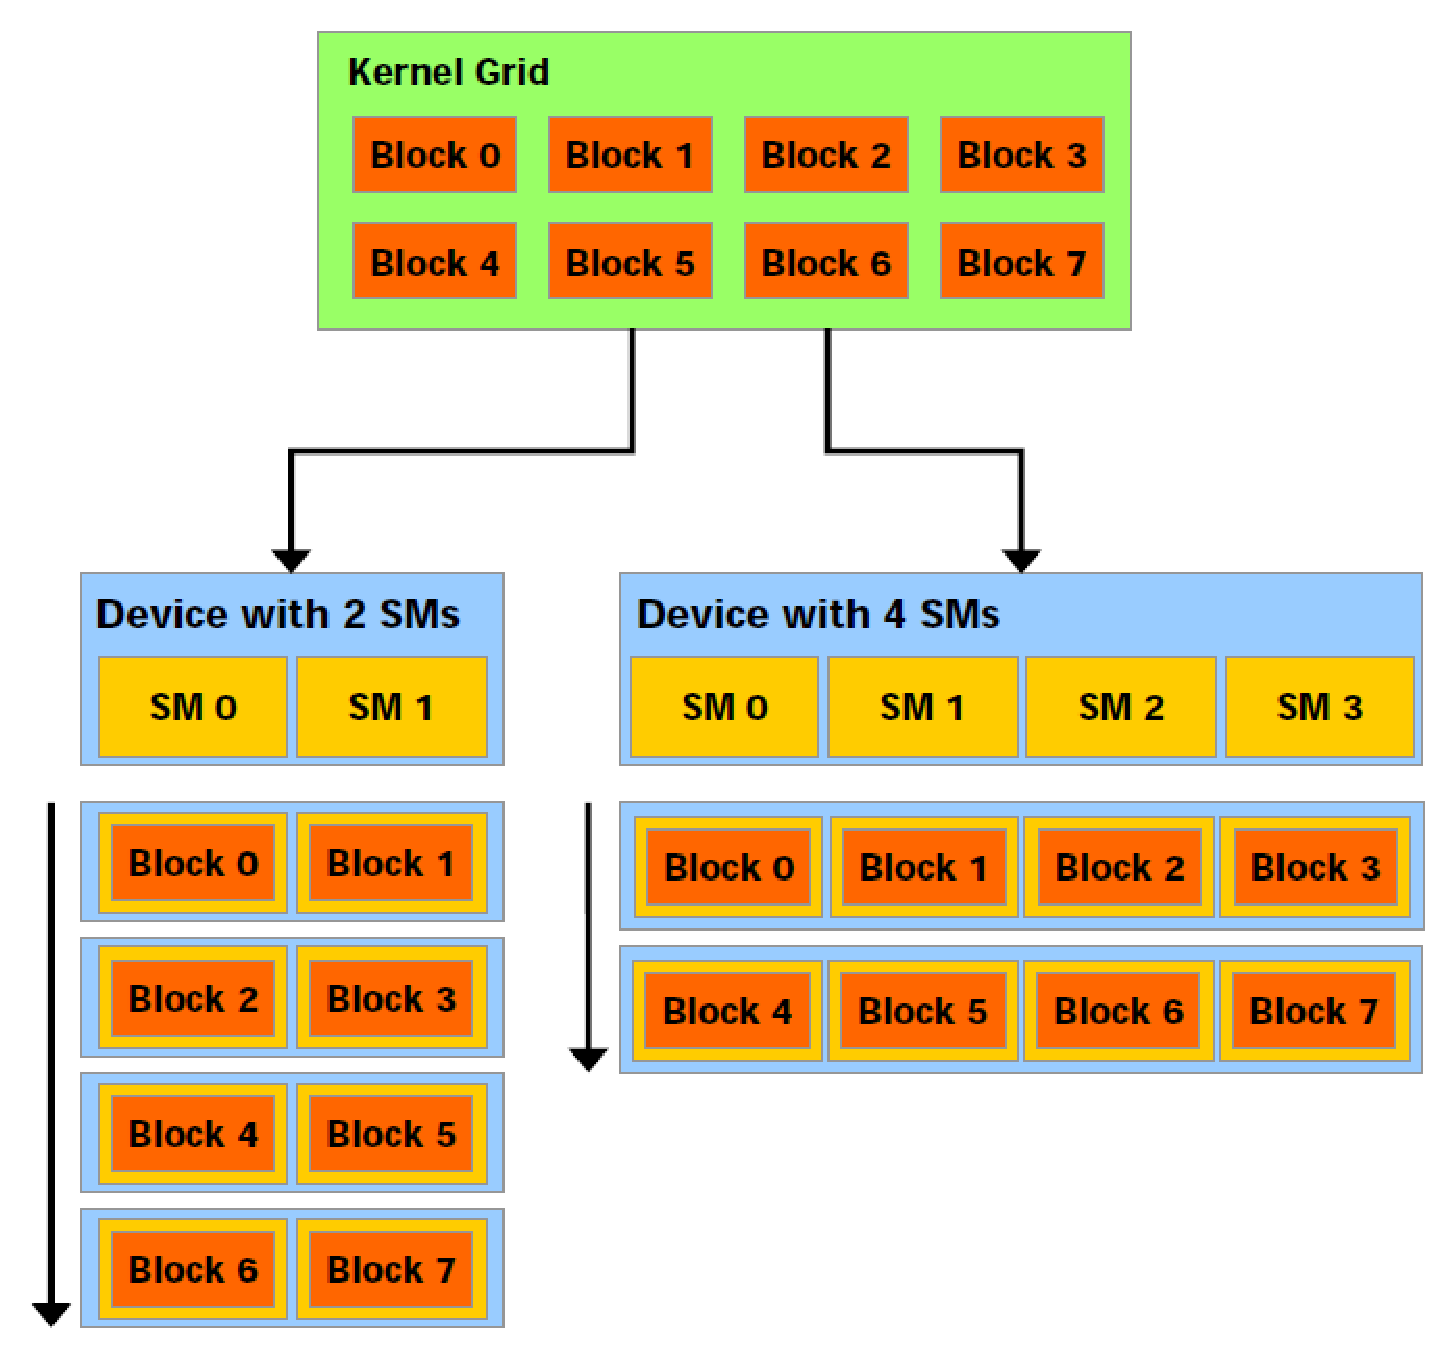
\includegraphics[height=6cm,
    angle=0]{./images/grid_sm.eps}}
\caption{A device with more SMs can execute a grid faster}
\label{fig:grid_sm}
\end{figure}


\begin{enumerate}
\item In CC 1.x, each SM has 8 scalar processor (SP), 2 special
  function units, a multithreaded instruction unit (warp scheduler),
  and an on-chip shared memory.
\item In CC 2.0, each SM has 32 scalar processor (SP), 4 special
  function units, two warp scheduler, an on-chip shared memory, L1/L2
  cache. 
\end{enumerate}
To allow multiple threads of a kernel run concurrently, Tesla card
employs the new architecture SIMT (single-instruction, multiple
threads). No matter how many threads in a thread blocks, each SMs
execute threads in groups of 32 threads, called {\bf warp}. Threads in
a warp execute the same instruction at a time. So, it's best if all
threads in a warp agree on their execution path. The difference in the
execution path occur only in conditional branch. That's why
conditional statement is limited in kernel as it slows down the
execution. Currently, at most one IF statement is allowed. If this
happen, the warp serially execute each branch path taken. Suppose it
has two path, the it execute threads follow path A first, then to
threads follow path B. When all paths in all threads of that warp
complete and the threads converge to the same execution path again,
the parallel execution continues.

{\bf NOTE}: Execution in different warps are independent. Thus, for
optimized organization, the threads in a thread block is often chosen
to be a multiply of 32.

Normally, one thread processes one data element, e.g. pixel in an
image, a voxel in a volume, a cell in a grid-based computation. 
As mention earlier, this can be other choices. 


\section{Data scope}
\label{sec:data-scope}

Sect.~\ref{sec:variables-1} describes how to declare a variable on
different memory spaces. This section will tell you whether the scope
of these variables are within threads, thread blocks, kernels, or the
whole program.

\begin{enumerate}
\item Each thread has its own memory (data is saved in registers or on
  global device memory)

\item Threads in the same block has a shared
  memory\footnote{show latency memory near each processor core (much
    like an L1 cache)},
  to which the threads need to synchronize using \verb!SYNCTHREADS()!
  when it is read or write.

\item Threads in different blocks can only share data via device
  memory space. 

\item Host subprogram and Kernel can only shared data by copying back
  and forth between device memory space vs. host memory space.

\item \textcolor{red}{Since CC 2.0 (Fermi GPU)}, L1/L2 caches are
  available. If the threads need to access device global memory a lot,
  it's better to cache the data to L1/L2 cache memory (this is managed
  by the system). Data on L1 cache is shared by threads on a SM; while
  data on L2 cache is shared by threads on any SM. You can adjust the
  memory for L1 between 16KB (default) or 48KB, depending on the
  kernel computation. Which data to be cached is hardware-managed.
\end{enumerate}

\begin{figure}[hbt]
  \centerline{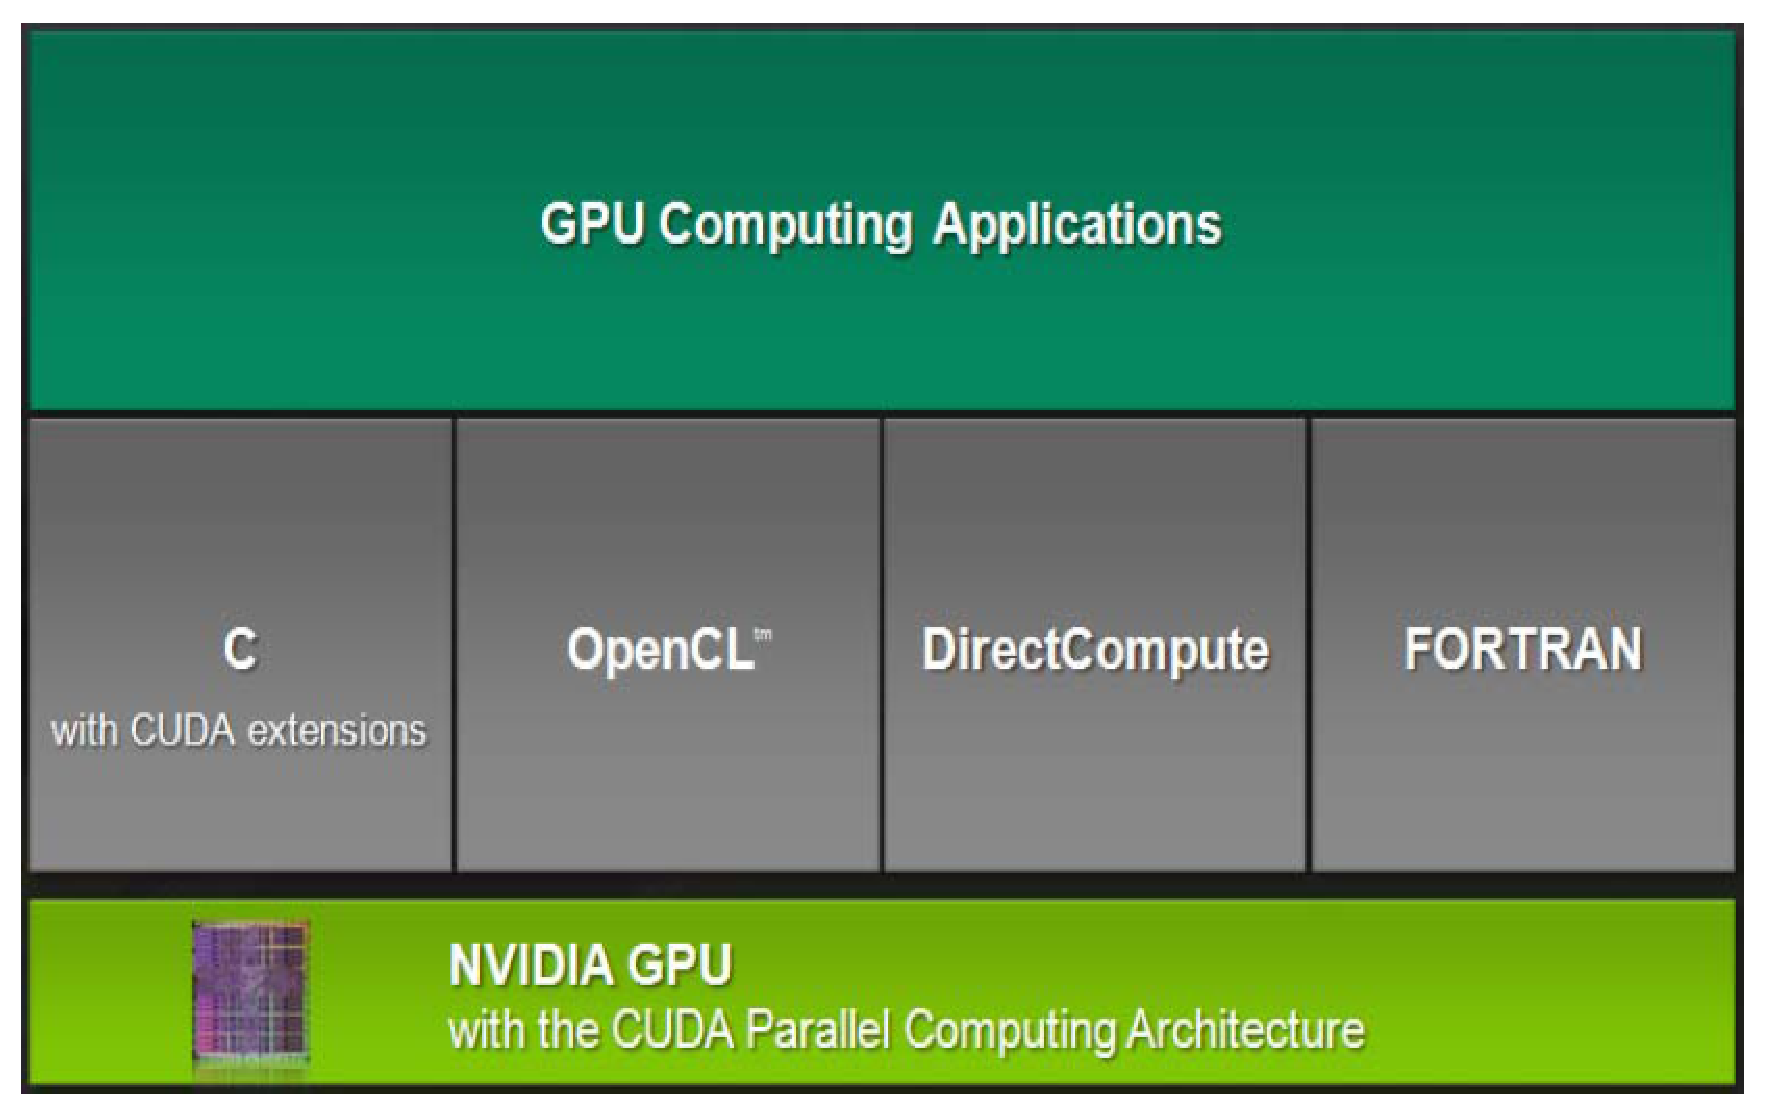
\includegraphics[height=5cm,
    angle=0]{./images/cuda_gpu.eps}}
  \caption{Diagram of how different languages access to GPU computing
    power}
  \label{fig:cuda_gpu}
\end{figure}

{\bf What we can do from host side?}
\begin{enumerate}
\item Directly access data on the {\it host main memory}.
\item Copy data back from and to {\it device global memory}
\item Set the values in the {\it device constant memory}
\end{enumerate}

Accessing to device memory is slower than accessing to the host memory
from host side, as it requires DMA access.

{\bf What can we do from device side?}
\begin{enumerate}
\item All threads can read data from or write data to
  {\it device global memory}
\item Data in the {\it device constant memory} must be initialized in
  the host program, and read-only in kernels.
\item Data in the {\it device constant memory} is read-only and often
  limited in size (16KB in Tesla 2nd gen; and configurable between
  16KB and 48KB in Fermi which affect L1 cache)

\item Threads in the same thread block can share data in {\it device
    shared memory} which has the lifetime of the thread block.
\item Each thread may have its own {\it private local memory} which
  can be either {\bf processor registers} (Sect.\ref{sec:register-files}) or
  {\bf global device memory}. It's best to keep data in
  processor registers, as it provides extremely fast speed (almost zero
  latency), yet limit to size. So, it's best to organize your kernel so that it use small
  enough amount of data. 
\end{enumerate}

\section{Synchronous data transfer}
\label{sec:cudaf_synch_datacopy}

\subsection{Data transfer host $\leftrightarrow$ device}
\label{sec:data-transfer-host}

%\subsection{Data in device constant memory}
%\label{sec:data-device-constant}

Typically, data on GPU is in global memory that we want tod deal with.
However, we can also use the assignment statement as mentioned in that for
device global memory to apply for data on constant memory.

%\subsection{Data in device global memory}
%\label{sec:data-device-global}

\subsubsection{Assignment statement}
\label{sec:assignment-statement}

One side is data on device, and the other side is data on host memory,
you can achieve data transfer using a simple assignment operator and
is synchronous
\begin{lstlisting}
A = Adev
Bdev = B
\end{lstlisting}
If you are in the host subprogram and have two variable of the same
type; one is declared in host memory and the other is declared
in {\bf device global memory}; you can simply use assignment for data
transfer from host memory to device global memory.

The left hand side can be a variable, a device array, or array
section; correspondingly, the right hand side can be a variable, a
host array or array section. 

% The reverse condition is applied for copying data from device global
% memory to host memory. 

\begin{framed}
  IMPORTANT: Using assignment, data is transferred via CUDA stream
  zero. As a result, this is a {\bf synchronous} operation which means
  it will wait for all kernels and any data transfer from any other
  stream to be completed.

  If we want to use asynchronous data transfer to enable the
  overlapping with other data copies or kernel execution, we need to
  have the data on the host paged-lock memory.
\end{framed}

\subsubsection{Implicit expression}
\label{sec:implicit-expression}

In an expression, the rule of thumb is that
{\it the operation must be performed on host memory}. So, if there is
a device variable in the expression, the compiler will automatically
generate a temporarily variable on host memory to store the data copy
from the device.
\textcolor{red}{Thus, in CUDA Fortran, there is AT MOST one device
  memory variable in the expression}.
\begin{lstlisting}
// COMPILE ERROR if both adev and bdev on device
a = adev + bdev
\end{lstlisting}

If you have more than one device memory variables that want to involve
in the expression, you need to explicitly break the expression into
two or more separate expressions, as given
\begin{lstlisting}
a = adev
a = a + bdev
\end{lstlisting}

\begin{framed}  
  \textcolor{red}{Elemental transfer is supported by the language
    itself, yet the performance is very poor}, i.e. copy a scalar
  variable across the CPU-GPU connection.
  
  The performance of array slices transfer depends upon various
  factors, i.e.  the size of the slices, the amount of contiguous data
  and the implementation.
\end{framed}



\subsubsection{CUDA Runtime APIs}
\label{sec:cuda-runtime-apis}

You can use \verb!cudaMemcpy(dest, src, count [, kdir])! function;
with \verb!count! is in number of elements, not in bytes like CUDA C.
\begin{lstlisting}
real, device :: wrk(1024)
real :: cur(512)

istat = cudaMemcpy ( wrk, cur, 512)
\end{lstlisting}
We don't need the fourth argument as the direction is known in CUDA
Fortran. If we want to use, they can be \verb!cudaMemcpyHostToDevice!,
...

\subsection{Using Runtime routines}
\label{sec:runtime-routines}

PGI Fortran provides the interfaces to the CUDA C runtime APIs,
e.g. \verb!cudaMemCpy()!. However, the third argument is the number of
elements by default, not the number of bytes as in CUDA C.
\begin{lstlisting}
real, device :: wrk(1024)
real :: curr(512)

istat = cudaMemCpy(wrk, cur, 512)
\end{lstlisting}

\verb!cudaMemcpy2D()! 
% They can do all the task related to copy data from host to device,
% from device to host, or fro one device array to another.


\subsubsection{Copy vector or scalar data}
\label{sec:copy-data}

You can transfer data from host to device, from device to host, or
from one device array to another. 
\begin{lstlisting}
integer function cudaMemcpy(dst, src, count, kdir)
\end{lstlisting}
We use \verb.cudaMemcpy(). to copy data with
\begin{itemize}
\item \verb!dst, src! can be in device, or host memory
\item if \verb!dst, src! is a scalar or an array of
  \hyperref[sec:datatype-data-device]{supported types}
  \begin{enumerate}
  \item \verb!count! is the number of elements
  \item \verb!kdir!  is optional since, in Fortran, the direction of
    copying is explicitly declared. If specified, it must be one of
    the defined enums
  \begin{enumerate}
  \item \verb!cudaMemcpyHostToDevice!
  \item \verb!cudaMemcpyDeviceToHost!, or
  \item \verb!cudaMemcpyDeviceToDevice!
  \end{enumerate}
  \end{enumerate}
\item if \verb!dst, src! is of type \verb!TYPE(C_DEVPTR)! or
  \verb!TYPE(C_PTR)!. 
  \begin{enumerate}
  \item \verb!count! is the number of bytes
  \end{enumerate}
\end{itemize}

% between host and device. The
% third argument is the number of elements, not bytes. 
{\bf Example}: 
\begin{lstlisting}
real, device :: wrk(1024)
real cur(512)
istat = cudaMemcpy(wrk, cur, 512)
\end{lstlisting}

An alternate is to use \verb!cudaMemcpyToArray! to copy array data
from host to the device, \verb!cudaMemcpyFromArray! to copy array data
from the device to host, and \verb!cudaMemcpyArrayToArray! to copy
array data from the device to device.

\begin{lstlisting}
integer function cudaMemcpyToArray(dsta, dstx, dsty, src,
count, kdir)
   type(cudaArrayPtr) :: dsta
   integer :: dstx, dsty, count, kdir

integer function cudaMemcpyFromArray(dst, srca, srcx, srcy,
count, kdir)
   type(cudaArrayPtr) :: srca
   integer :: dstx, dsty, count, kdir

integer function cudaMemcpyArrayToArray(dsta, dstx, dsty,
srca, srcx, srcy, count, kdir)
   type(cudaArrayPtr) :: dsta, srca
   integer :: dstx, dsty, srcx, srcy, count, kdir
\end{lstlisting}


\subsubsection{Copy 2D array data}
\label{sec:copy-2d-array}

You can transfer data from host to device, from device to host, or
from one device array to another. 
\begin{lstlisting}
integer function cudaMemcpy2D(dst, dpitch, src, spitch,
width, height, kdir)
\end{lstlisting}
with
\begin{itemize}
\item \verb!dst, src! can be in device, or host memory
\item if \verb!dst, src! is an array of
  \hyperref[sec:datatype-data-device]{supported types}
  \begin{enumerate}
  \item \verb!width, height! is the number of elements, in each
    direction
  \item \verb!kdir!  is optional since, in Fortran, the direction of
    copying is explicitly declared. If specified, it must be one of
    the defined enums
  \begin{enumerate}
  \item \verb!cudaMemcpyHostToDevice!
  \item \verb!cudaMemcpyDeviceToHost!, or
  \item \verb!cudaMemcpyDeviceToDevice!
  \end{enumerate}
  \end{enumerate}

  For better performance, Fortran may automatically pad the data, the
  padded width (in terms of number of elements) is returned in
  \verb!dpitch, spitch!.

\item if \verb!dst, src! is of type \verb!TYPE(C_DEVPTR)! or
  \verb!TYPE(C_PTR)!. 
  \begin{enumerate}
  \item \verb!width, height! are the number of bytes
  \end{enumerate}

\end{itemize}


An alternate is to use \verb!cudaMemcpy2DToArray! to copy array data
from host to the device, \verb!cudaMemcpy2DFromArray! to copy array
from the device to host, and \verb!cudaMemcpy2DArrayToArray! to copy
array data from device to device.
\begin{lstlisting}
integer function cudaMemcpy2DToArray(dsta, dstx, dsty, src,
spitch, width, height, kdir)
   type(cudaArrayPtr) :: dsta
   integer :: dstx, dsty, spitch, width, height, kdir

integer function cudaMemcpy2DFromArray(dst, dpitch, srca,
srcx, srcy, width, height, kdir)
   type(cudaArrayPtr) :: srca
   integer :: dpitch, srcx, srcy, width, height, kdir

integer function cudaMemcpy2DArrayToArray(dsta, dstx, dsty,
srca, srcx, srcy, width, height, kdir)
   type(cudaArrayPtr) :: dsta, srca
   integer :: dstx, dsty, srcx, srcy, width, height, kdir
\end{lstlisting}


\subsubsection{Copy 3D array data}
\label{sec:copy-3d-array}

\begin{lstlisting}
integer function cudaMemcpy3D(p)
    type(cudaMemcpy3DParms) :: p
\end{lstlisting}


\subsubsection{Set value to a vector or scalar device data}
\label{sec:set-value-vector}

You can set a location or a 1D array to a specified single value using
\begin{lstlisting}
integer function cudaMemset(devptr, value, count)
\end{lstlisting}
with \verb!devptr! can be 

\begin{itemize}
\item can be a device scalar or a 1D device array of a
  \hyperref[sec:datatype-data-device]{supported types}; then
  \verb!count!  is the number of elements

\item of \verb!TYPE(C_DEVPTR)! datatype, then \verb!count! is the
  number of bytes, then the lowest byte of \verb!value! is used to
  assigned to \verb!count! bytes of \verb!devptr!.

\end{itemize}

{\bf NOTE}: \verb!value! must match in {\it kind} and {\it type} of
elements of \verb!devptr!.


\subsubsection{Set value to a 2D array device data}
\label{sec:set-value-2d}

\begin{lstlisting}
integer function cudaMemset2D(devptr, pitch, value, width,
height)
\end{lstlisting}
with \verb!devptr! can be
\begin{itemize}

\item a 2D device array of a
  \hyperref[sec:datatype-data-device]{supported type}; then
  \verb!width, height!  is the number of elements on each direction.

  For better performance, CUDA Fortran may pad the data, and the
  padded width (in terms of number of elements) is returned in
  \verb!pitch!  (integer).
\item of \verb!TYPE(C_DEVPTR)! datatype, then
  \verb!pitch, width, height! express the number of bytes, and the
  lowest byte of \verb!value! is used to assigned to each byte of
  \verb!devptr!.

\end{itemize}
and \verb!value! must match in {\it kind} and {\it type} of elements
of \verb!devptr!. 

\subsubsection{Set value to a 3D array device data}
\label{sec:set-value-3d}

\begin{lstlisting}
integer function cudaMemset3D(pitchptr, value, cext)
    type(cudaPitchedPtr) :: pitchptr
    integer :: value
    type(cudaExtent) :: cext
\end{lstlisting}

\subsection{Data transfer device $\leftrightarrow$ device}
\label{sec:data-transfer-device}

In CUDA Fortran of PGI 10.4, we can not use assignment to 
copy data from one device memory variable to another device memory
variable. The only way is to use CUDA runtime API 
\verb!cudaMemcpy(a_dev,b_dev,...)!. 

In PGI 10.5, device to device copies using assignment will be supported, i.e.
where both the left-hand side
and right-hand side are data on device. 
\begin{lstlisting}
Adev = Bdev
\end{lstlisting}


\subsection{Tips \& Tricks}
\label{sec:tips--tricks}

\begin{figure}[hbt]
  \centerline{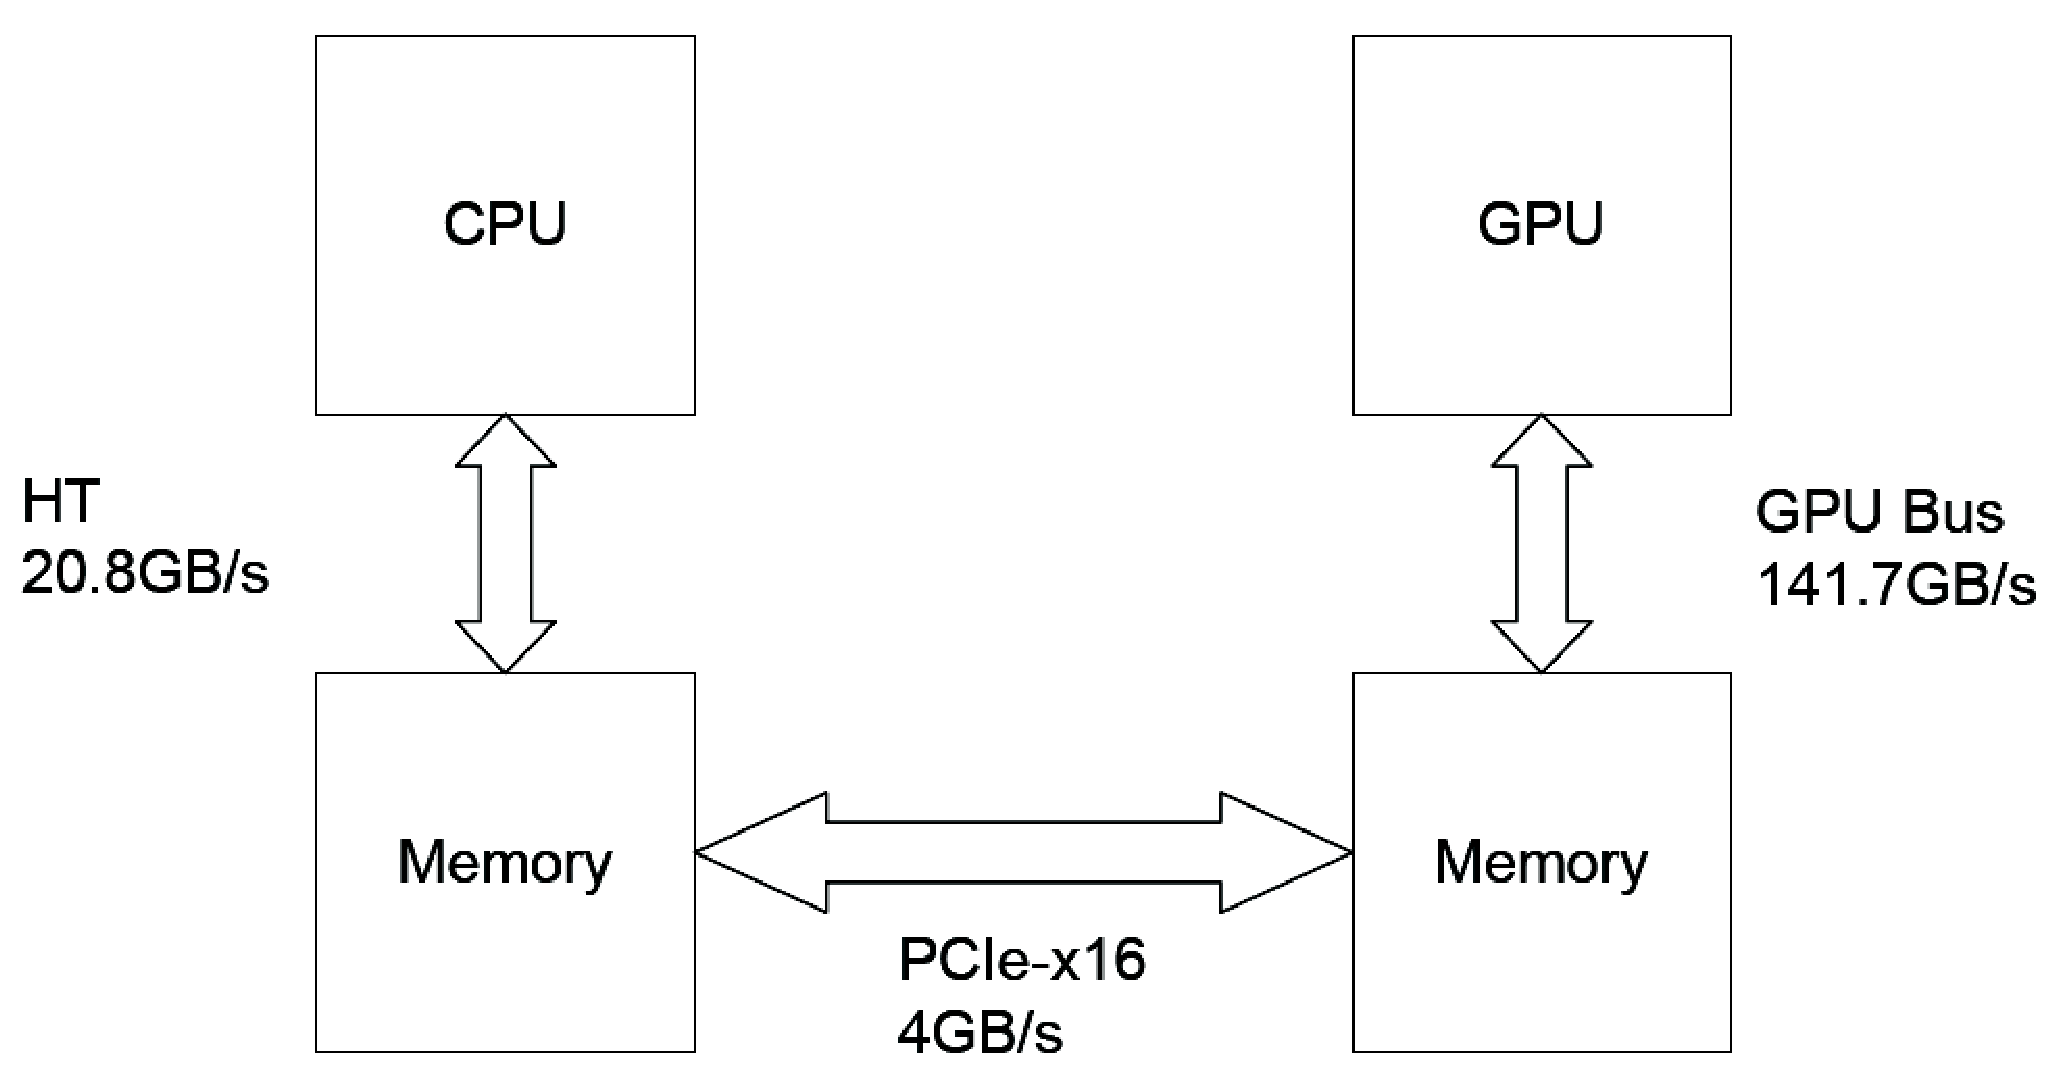
\includegraphics[height=5cm,
    angle=0]{./images/cuda_datamodel.eps}}
\caption{Data transfer information}
\label{fig:cuda_data}
\end{figure}

As shown in Fig.~\ref{fig:cuda_data}, it's quite expensive when
copying data back and forth device and host. So, if you're in a loop,
you should keep computed data on device memory for a number of
iteration, say 1000, before copying back to CPU.
\begin{verbatim}
Transfer data to GPU
For t=1 to 1000000:
  Run the code on the GPU
  If (t%100)==0 then
     transfer data to CPU
     Print/save data on CPU
  endif
  Transfer data to GPU CPU
endfor
\end{verbatim}

\section{Asynchronous data transfer}
\label{sec:cudaf_asynch_datacopy}

Since CUDA 3.x, we can use asynchronous data transfer to hide dead time by
overlapping kernel execution and data copy. The limitations are:
\begin{enumerate}
  \item Data on host must be allocated on {\bf pinned} (page-lock) memory space. 
  \item Create a CUDA stream different than that using for the kernel
  \item Call the runtime API \verb!cudaMemcpyAsync()! with the designed CUDA
  steram
\end{enumerate}

\begin{lstlisting}
REAL, DIMENSION(:), ALLOCATABLE, PINNED :: a_pin
REAL, DIMENSION(:), ALLOCATABLE, DEVICE :: a_dev

ALLOCATE(a_pin(1000))
ALLOCATE(a_dev(1000))

cudaerr = cuda
\end{lstlisting}

NOTE: Asynchronous data transfer typically requires using double buffering,
where the kernel update data in the first buffer, while the data in the second
buffer is copied. In the next loop, data in the second buffer is updated by the
kernel, while that in the first buffer is copied back. 

\subsection{Shared pinned memory between processes/threads}
\label{sec:cudaf_shared_pinned_mem}

Using asynchronous data transfer requires using pinned memory. However, pinned
memory cannot be shared between threads/processes. CUDA 4.0 comes up with a new
API that allows you to register that allocated pinned memory to use in one
thread with \verb!cudaHostRegister()! and then release if after finishing using
\verb!cudaHostUnregister!. However, in CUDA Fortran, this feature is hard to
implement. At first, due to the limitation of the API, which requires the data
to be allocated on pinned memory aligned on a 4K boundary, and a size of the
data must be a multiple of 4K. 

In general, the address of the buffer is that not accessible by Fortran, so from
the concept of the language, this is almost impossible to achieve. However,
there are some platform-specific functions that can allocate memory aligned on
this boundaray, e.g. \verb!posix_memalign! of Linux. Then, PGI CUDA Fortran has
plan to create the ``ALIGN'' qualifier on the ALLOCATE() statement, that will
sit on top of these platform-specific rountine to return the aligned buffer
area. However, there is no information when this is available; maybe until PGI
v12.0. For now, padd your data to the size of 4K multiple, and use the platform
specific routine to allocate the data, next pass the pointer to Fortran
using \verb!c_ptr! or \verb!c_f_pointer! (via \verb!iso_c_binding! module) and
use CUDA C runtime API \verb!cudaHostRegister()! to get access to it. 

Read more on CUDA C part (Sect.\ref{sec:cudac_share_pinned_mem}).

\section{Call a kernel subroutine}
\label{sec:call-kernel}

To call a kernel, we need to specify the execution configuration which
defines the dimension and extent of the grid and thread block that
will execute the kernel. For a more detail discussion on choosing the
blocks size and grid size, read Sec.~\ref{sec:kern-exec-conf}.

We may also specify the dynamic shared memory extent, in bytes, and a
stream identifier, to support concurrent stream execution on the
device.

\begin{lstlisting}
call kernel<<<grid,block[,bytes[,streamid]]>>>(arg1,arg2,...)
\end{lstlisting}
with 
\begin{itemize}
\item \verb.grid., \verb.block. can be an integer (for 1D) or a
  variable of derived type \lstinline{type(dim3)} (for 1D, 2D or
  3D). Limitations: 
  \begin{enumerate}
  \item maximum extent for dimension x, y, and z in a block is 512,
    512, and 64 respectively. The restriction is that: number of
    threads per block $\le$ 512 (\verb!sm_12, sm_13!), while it is
    1024 in Fermi (\verb!sm_20!).
  \item the grid has maximum 2D, then \verb.grid%z. must
    be one with the maximum extent for the first two dimension in a
    grid is 65535. So the maximum dim is $65535\times 65535\times 1$.
  \end{enumerate}
  Based on the current CUDA architecture, each kernel correspond to
  one grid. Up to \verb!sm_13!, each device only process one kernel at
  a time. Since \verb!sm_20!, each device can process maximum 16
  kernels in a single program. However, kernels from two different
  programs need to run sequentially. 
\item \verb.bytes. is a positive integer, which tell the number of
  bytes to be allocated for dynamic shared memory within a single
  thread block, in addition to the statistically allocated shared
  memory within a single thread block. This dynamic shared memory is
  used for any \hyperref[lab:assa]{assumed-sized shared array} in
  thread block (in C, we call it external array).
\item \verb.streamid. is a non-negative integer, which specify the
  stream to which this call is associated. Different stream has
  different priority in using GPU (read
  \hyperref[sec:conc-stre-exec]{here} for more information)
\end{itemize}

{\bf IMPORTANT}: When you want to call a kernel subroutine from a host
subprogram, and the actual arguments are locating on the host memory,
you need to call CUDA Fortran API for copying them to the device
memory first and then passing these new variables (which are declared
using appropriate attributes to be introduced later) to the kernel
subroutine (read more in Sec.~\ref{sec:passing-data-kernel}).

\subsection{Passing data to kernel subroutine}
\label{sec:passing-data-kernel}

In Fortran, by default, dummy arguments are passed by reference. This
apply for parameters in a kernel subroutine also. This means the
actual argument must be stored on the device memory first and its
address is passed to the subprogram. In other words, before calling to
a device subroutine, you need to put all argument in the device memory
first using appropriate CUDA Fortran APIs, and then pass the new
variables to the device subroutine.

In certain cases, e.g. for scalar arguments, you may want to pass by
value, you can do this by adding the value attribute to the variable
declaration in the device subroutine
\begin{lstlisting}
attributes(global) subroutine madd( a, b, n )
   real, dimension(n,n) :: a, b
   integer, value :: n
\end{lstlisting}
Here, the actual arguments to the two dummy matrices a and b still
need to be set up to reside on the device before the call to this
device subroutine.

Inside a kernel, you can define local variable using either of the
following attribute
\begin{enumerate}
\item no attribute is used: data reside in global device memory by
  default % private local variable is stored in
  % registers (if it is scalar and allowed for a small number of
  % scalar), otherwise, will reside in global device memory.
\item \verb!value! : data with \verb!value! attribute are usually
  scalar, and dummy arguments, from which the actual argument doesn't
  have to reside on device memory, i.e. the data of actual argument
  can be in host memory, and will be copied automatically to the
  device memory.

\item \verb!global! : data is forced to reside in the global device
  memory (accessible by all threads in all blocks)

\item \verb!shared! : data is forced to reside in the thread shared
  memory, (accessible by all threads in a single block). If it is an
  locally defined array (not argument passing), it can be either fixed
  size or assumed-size array.

  {\bf NOTE}: a shared array that is not a dummy argument may be
  declared as an assumed-size array, i.e. the last dimension has an
  asterisk as the upper bound.The size (in bytes) for this array is
  determined at runtime and is specified by the third argument to the
  chevron syntax. When there are more than one shared variables like
  this, they all share the same starting address memory; thus
  modifying one may alter the value of the others. Programmers need to
  handle with care if using multiple shared variables.

\item \verb!constant!: data is forced to reside in constant space
  (limit to 64KB totally), as data cannot be modified inside the
  kernel, this data is often passed by argument or defined inside a
  module so that all kernel can access.
\end{enumerate}

NOTE: Access to constant memory is slow as access to global device
memory. Only to access local and shared are fast.


Which kind of data can be passed to kernel?
\begin{enumerate}
\item \verb!device!: data declared in the host subprogram, which can
  be either scalar or array (can be allocatable), when passing as
  argument, the dummy argument must be declared with \verb!device!
  attribute. 
\item \verb!constant!: this data is read-only in kernel subprogram
\item \verb!shared! :
  \textcolor{red}{valid only when data is passed from a device
    subprogram to another device subprogram}. Both dummy argument and
  actual argument must have \verb!shared! attribute.
\end{enumerate}

Which kind of data CANNOT be used in a kernel?
\begin{enumerate}
\item Any variable (scalar or array) regardless of their location
  (host or device memory) defined in a higher scope and is not passed
  via arguments.

\item \verb!pinned!: data declared in the host subprogram will reside
  in the page-locked host memory, suitable for data that is transfer
  back and forth the kernel very often and can be asynchronous.

\end{enumerate}

Which attribute CANNOT be used to define data outside of a kernel?
\begin{enumerate}
\item \verb!shared!: Only valid to define variables inside a kernel
\end{enumerate}

For other restrictions on device subprogram and kernel subroutine, read
Sec.~\ref{sec:restriction}.

\subsection{Concurrent host and device execution}
\label{sec:conc-host-device}

By default, calling to a device subprogram only put that kernel into a
queue, waiting for execution on the device, and the control is return
to the host subprogram immediately. Then, both the device and host
code execute concurrently. It means that the host can then execute and
put more kernels to the queue. 

However, this is dangerous as the host may modify device or constant
data unexpectedly. So, when a host subprogram need to access a
critical data, it's better to call the function
\verb.cudaThreadSynchronize(). before accessing to the data.

\begin{lstlisting}
call foofunc<<<1, 5>>>(arg1,arg2)

// host code that do not modify device data
// being used by foofunc.

cudaThreadSynchronize()
// host code that use device data
\end{lstlisting}

CUDA Fortran API \verb.cudaThreadSynchronize(). block the execution of
host subprogram until all preceding kernels and operations are
complete. It may return an error code that tells if one of the
preceding kernel operations fail. 

\subsection{Concurrent stream execution (CUDA stream)}
\label{sec:conc-stre-exec}

Any operations using the device, e.g. copy to and from the device or
running a kernel... are implemented using {\bf stream queue}. Thus, an
operation is put to the stream queue and waiting for its turn when all
previous operations have been completed.

By default, these operations are put to the default stream queue, and
thus sequentially executed. To improve the concurrency; we need to put
these operations into different stream queues. The default stream,
when no stream ID is specified, is zero. You can specify the stream
ID, via the chevron syntax when calling to a kernel. Stream zero has
the lowest priority, i.e. it begin only after all preceding operations
on all queues are complete, and no subsequent operations on any queue
will begin until the stream zero operation is complete.

Using multiple stream queues, there is no guarantee in the order of
the operations in the order for kernel residing on different
queues. So, it's important to put kernels that need to be executed in
order in the same stream queue; and those are supposed to be
independent can be put into different stream queues. 

For example: you have 2 copies of data \verb!a1, a2!. Basically, a1
and a2 are two copies at time t and $t-\delta t$. So, we use a2 to
calculate a1
\begin{lstlisting}

if (isEven .eq. .TRUE.) then 
   // calculate a1 
   call kernel<<<grid, block, 0, stream0>> (a1, a2, ...)
   copy(a_host, a2)
else 
   // calculate a2 
   call kernel<<<grid, block, 0, stream0>> (a2, a1, ...)
   copy(a_host, a1)
endif   
   _synchronize();
\end{lstlisting}


% \section{Synchronization}
% \label{sec:synchronization}

% \subsection{Between threads}
% \label{sec:between-threads}




\subsection{Variable usage}
\label{sec:variable-usage}

% \textcolor{red}{An allocatable device array MUST NOT be used as global
%   variable, i.e. whenever a kernel need to use it must be passed via
%   subprogram arguments.}
(FIXED in PGI 10.4)
\st{An allocatable device array MUST NOT be used as global variable,
  i.e. whenever a kernel need to use it must be passed via subprogram
  arguments. Otherwise, runtime error may occur, as given.}
% \begin{verbatim}
% copyout Memcpy FAILED:4  
% \end{verbatim}
% and the compiling status is something like 
% \begin{verbatim}
% : warning: cast to pointer from integer of different size
% : cannot tell what pointer points to, assuming global memory space
% \end{verbatim}
Allocatable device array defined in a module, which contains global
subprogram, can now be used in any host subprogram that use the
module, and the global subprograms in the module.


\textcolor{red}{Even static device data SHOULD NOT be defined in module
  region, as passing such data to a device subprogram from a host
  subroutine can cause this runtime error (no compiling warning)}
\begin{verbatim}
copyout Symbol Memcpy FAILED:4   ! this is unknown reason
\end{verbatim}


\subsection{Restriction}
\label{sec:restriction-1}

\subsubsection{In a host subprogram}
\label{sec:host-subprogram}

Device variable (array) can only be used 
\begin{enumerate}
\item In declaration statement
\begin{lstlisting}
integer, device:: a
\end{lstlisting}
\item As a dummy argument defined in a host subprogram
\item It may have ALLOCATABLE attribute, or adjustable extent.
\item In \verb!allocate()! or \verb!deallocate()! statement
\item As an actual argument to \verb!allocated()! intrinsic function
\item As an actual argument to a kernel subroutine
\item As an actual argument to another host subprogram (or runtime API
  call)
\end{enumerate}

Constant variable can only be used
\begin{enumerate}
\item In declaration statement
\item As the source or destination to data transfer statements
\item As an actual argument to another host program
\item As an dummy  argument to another host program
\end{enumerate}


\subsubsection{Datatype for data on device memory}
\label{sec:datatype-data-device}

Data defined with \verb!shared!, \verb!constant!, \verb!device!
attributes or defined in a {\it device subprogram} is limited to the
following datatypes:
\begin{enumerate}
\item integer 
\item logical
\item real
\item double precision
\item complex
\item character(len=1)
\end{enumerate}

They may be of derived type if the members are of intrinsic datatypes
given above or of a legal derived datatype. This is the derived type
defined in \verb!cudafor! module
\begin{lstlisting}
type(dim3)
  integer(kind=4) :: x, y, z
end type
\end{lstlisting}



\section{Using Fortran CUDA APIs}
\label{sec:using-fortran-cuda}

Many Fortran CUDA APIs can take {\it device} arrays as arguments.
With the support of Fortran 2003:
\begin{enumerate}
\item some can take C types, provided through the module
  \verb!iso_c_binding!, as arguments.

\item In addition to the derived type \verb!TYPE(C_PTR)! used for C
  pointer, a C device pointer is of type \verb!TYPE(C_DEVPTR)! which
  is defined in the \verb!cudafor!  module.
\end{enumerate}

{\bf IMPORTANT}: It's recommended to use \verb!TYPE(C_PTR)! and
\verb!TYPE(C_DEVPTR)!, as well as consistency check between Fortran
device arrays and host arrays. 

{\bf Create a device pointer to a Fortran device array using
  \verb!TYPE(C_DEVPTR)!}:
\begin{enumerate}
\item use the subroutine \verb!c_f_pointer()! from the module
  \verb!iso_c_binding! (since Fortran 2003)
\begin{lstlisting}
use iso_c_binding
TYPE(C_DEVPTR) :: arg1
real, allocatable, dimension(:,:), device :: arg2
integer, dimension(2) :: shape

shape = (/ 2, 5 /)
c_f_pointer(arg1, arg2, shape)
\end{lstlisting}

\item We can also use \verb!C_DEVLOC()! to create a type
  \verb!TYPE(C_DEVPTR)! that hold the C address of the Fortran device
  array argyment.
\end{enumerate}
Both of these two features are subjected to change when, in the
future, proper Fortran pointer to device array are supported.

\subsection{Allocate a vector}
\label{sec:allocate-vector}

\begin{lstlisting}
integer function cudaMalloc(devptr, count)
\end{lstlisting}
with \verb!devptr! can be
\begin{itemize}
\item an allocatable, 1D device array of a
\hyperref[sec:datatype-data-device]{supported type}; then \verb!count!
is the number of elements

\item of \verb!TYPE(C_DEVPTR)! datatype, then \verb!count! is the
  number of bytes. 

\end{itemize}

% For device array allocation only, a different way is to use CUDA
% Fortran API.
{\bf Example}:
\begin{lstlisting}
real, allocatable, device :: v(:)
istat = cudaMalloc(v, 100)
...
istat = cudaFree(v)
\end{lstlisting}
The runtime API \verb.cudaMalloc. and \verb.cudaFree. work like C's
malloc() and free() function. So, there is no automatic deallocation
and thus we need to manually and explicitly free the data when it is
unused.

\subsection{Allocate a 2D array}
\label{sec:allocate-2d-array}

\begin{lstlisting}
integer function cudaMallocPitch(devptr, pitch, width,
height)
\end{lstlisting}
with \verb!devptr! can be
\begin{itemize}
\item an allocatable, 2D device array of a
  \hyperref[sec:datatype-data-device]{supported type}; then
  \verb!width, height!  is the number of elements on each direction.

  For better performance, CUDA Fortran may pad the data, and the
  padded width (in terms of number of elements) is returned in
  \verb!pitch!  (integer).
\item of \verb!TYPE(C_DEVPTR)! datatype, then
  \verb!pitch, width, height! express the number of bytes.
\end{itemize}

To free data, we need to use \verb!cudaFree(devptr)!. 

An alternate is to use \verb!cudaMallocArray! and
\verb!cudaFreeArray!.
\begin{lstlisting}
integer function cudaMallocArray(carray, cdesc, width,
height)
   type(cudaArrayPtr) :: carray
   type(cudaChannelFormatDesc) :: cdesc
   integer :: width, height

integer function cudaFreeArray(carray)
\end{lstlisting}


\subsection{Allocate a 3D array}
\label{sec:allocate-3d-array}

\begin{lstlisting}
integer function cudaMalloc3D(pitchptr, cext)
   type(cudaPitchedPtr), intent(out) :: pitchptr
   type(cudaExtent), intent(in) :: cext
\end{lstlisting}


An alternate is to use \verb!cudaMalloc3DArray!
\begin{lstlisting}
integer function cudaMalloc3DArray(carray, cdesc, cext)
   type(cudaArrayPtr) :: carray
   type(cudaChannelFormatDesc) :: cdesc
   type(cudaExtent) :: cext
\end{lstlisting}


\section{Thread and thread block}
\label{sec:thread-thread-block}

\begin{enumerate}
\item Maximum number of threads per thread block is 512 (for CC.1.x)
  and 1024 (for CC.2.0).
\item Maximum dimension of a thread block is
  $512\times512\times64$. However, due to the above restriction,
  i.e. $x\times y\times z \le 512$ (for CC.1.x) and $x\times y\times z
  \le 1024$ (for CC.2.0), we cannot get all dimension maximized at the
  same time. To maximum the usage of threads per thread block, we
  often choose $x,y,z$ so that $x\times y\times z = 512$ (on GPU of
  CC.1.x) or $x\times y \times z=1024$ (on GPU of CC.2.0). In
  addition, as threads are executed in group of 32 called {\it warps},
  the number of threads need to be a multiple of 32 also,
  i.e. $x\times y\times z \mod 32 = 0$.

  Here are some common choices for x, y and z (depending on the
  problem) for GPU of CC.1.x
\begin{verbatim}
        x     y   z
        512   1   1
        64    8   1
        16    32  1
        8     8   8
        16    16  1   ! = 256 < 512
\end{verbatim}
  As the number of registers is limited, and kernel intensively use
  register to store the data, kernel usage of registers also decide
  the choice of the block configuration. To get the information about
  kernel usage, compile with the compiler option
  \verb!--ptxas-options=-v!  (Read Sect.~\ref{sec:tuning-code})
\item A grid can be 1D or 2D in which the maximum for one dimension is
  65535.
  \begin{eqnarray}
    \label{eq:99}
    65,535\times 65,535\times 1
  \end{eqnarray}
\end{enumerate}

Read more in Sect.~\ref{sec:tuning-code}.

\section{Intrinsic functions}
\label{sec:intrinsic-functions-2}

Due to the certain limitations of the hardware of GPU compared to that
of CPU, not all Fortran intrinsic functions work well on GPU. Here is
the list of subroutine/functions that work well on GPU.

Upto Fortran 11.8. NOTE: When we say ``real'' it means both single and
double precision. 
\begin{verbatim}
func-name|| argument type

abs        integer, real, complex
aimag      complex
aint       real
anint      real
ceiling    real
cmplx      real, (real,real)
conjg      complex   --> find conjugate
dim        integer, real
floor      real
int        integer, real, complex
logical    logical
max        integer, real
min        integer, real
mod        integer, real
modulo     integer, real
nint       real
real       integer, real, complex
sign       integer, real
\end{verbatim}

If not mentioned, they only support ``real''.
\begin{verbatim}
acos
asin
atan
atan2       (real, real)
cos         real, complex
cosh
exp         real, complex
log         real, complex
log10       real
sin
sinh
sqrt        real, complex
tan
tanh
\end{verbatim}



\begin{verbatim}
bit_size
digits       integer, real
epsilon      real   --> return the smallest value larger than zero
huge         integer, real  --> return the largest value of that type
maxexponent
minexponent
precision
radix
range
selected_int_kind
selected_real_kind   (integer, integer)
tiny
\end{verbatim}


CUDA Fortran implement some reduction operations. 
\begin{verbatim}
all         if all threads in the block ....
any         if any thread in the block satisfies the condition
count       if a certain number of thread in the block satisfies the
            condition 
minloc
minval
product
maxloc
maxval
sum
\end{verbatim}

Random numbers are also supported
\begin{verbatim}
random_number       real
random_seed         integer
\end{verbatim}

See documentation of CUDA Fortran.

\section{Sync threads within a block}
\label{sec:synthreads-block}

If you want all threads in a block to reach a certain location before
they can proceed, you use \verb!syncthreads()! with no argument. This
will avoid potential read-after-write, write-after-read, or
write-after-write hazards when more than one threads within a block
access the same address in shared or global memory.
\begin{lstlisting}
... Step 1...
__syncthreads();
... Step 2...
\end{lstlisting}

IMPORTANT: You cannot put \verb!syncthreads()! (or functions of its
kind) inside an IF statement or loops. It means all threads must
execute it. 

There are other options are:
\begin{lstlisting}
syncthreads_count(int value)
   all threads must reach the same place; in addition, it returns the
   number of threads in the block that has 'value' is non-zero.
   
syncthreads_and(int value) 
   all threads must reach the same place; in addition, it evaluates
   the variable 'value' for all threads and return non-zero
   if-and-only-if all 'value' in all thread are non-zero
   
syncthreads_or
   all threads must reach the same place; in addition, it returns
   non-zero if at least one of 'value' is non-zero.
threadfence
threadfence_block
threadfence_system
\end{lstlisting}

Typically, we use sync threads when we want threads in the same thread
blocks reach a particular statement; regardless of whether we want them to wait
for data written out/read in or any thing else. However, when we want to make
sure data written by one thread is complete, and can be seen by other threads,
in the same or different thread blocks, we need to use memory fence. The function CUDA
provided for memory fence is \verb!threadfence()!
(Sect.~\ref{sec:memory-fences}). Here, in
order for new data to be seen by threads from other thread blocks, the data
need to reside globald device memory.

If we only need memory fence to apply for threads in the same block only (single
block communication), you can use \verb!threadfence_block()! instead.


\section{Memory fences}
\label{sec:memory-fences}

Typically, the execution of one block is independent from the others. However,
since CUDA 4.0, we can make sure data written by threads from one thread blocks
can be read-in properly from threads in another thread block. Using
\verb!threadfence()! is good for inter-block communications.
\begin{lstlisting}
voide threadfence()
\end{lstlisting}
enforces all threads in the block/grid to write data in their
(local/global) thread ID order (increasing), depending where the data
is written to (shared or global). After the call, 
\begin{itemize}
\item all global memory updates are visible to all threads in the
  device. 
\item all shared memory update are visible to all threads in the block
\end{itemize}
If we limit the constraint to threads in the same block, not between blocks, we
can use \verb!threadfence_block()!.

CUDA 4.0 another similar function, to extend the memory fence from shared/global
memory to pinned memory. So, by using \verb!threadfence_system()!, after this
call, it guarantees memory data access before the call is completed and thus
visible to
\begin{itemize}
\item all threads in the thread blocks for shared memory
\item all threads in the device for global memory
\item host threads for page-locked host memory
\end{itemize}

\begin{framed}
NOTE: If we use atomic functions, it implicitly guarantees read-mofiy-write of
the data. So we don't need to use thread fence. 
\end{framed}

\section{Warp-vote operations}
\label{sec:warp-vote-operations}


Another way of inter-thread communication, but not at the thread block
level, is using warp-vote operations. This will take affect for
threads in the same warp. 
\begin{itemize}
\item \verb!allthreads(expression)! return true if all threads in the
  warp evaluate `expression' to true
\begin{lstlisting}
if (allthreads(a(i) < 0.0) allneg = .true.
\end{lstlisting}


\item \verb!anythread()! returns
\item \verb!ballot()! 
\begin{lstlisting}
unsigned integer ballot (int value)
\end{lstlisting}
\end{itemize}


\section{Atomic function}
\label{sec:atomic-function-fcuda}

Atomic functions are important in parallel computing (e.g. parallel
sorting, reduction operations...). It guarantees parallel threads to
read/write on shared data correctly. It means that all stages of an
operation, including read + modify + write, are performed without
interruption from other threads. Example of atomic functions are min,
max, compare-and-swap. A section for CUDA C is given in
Sect.\ref{sec:atomic-functions}.

\begin{framed}
  \textcolor{red}{PGI v10.x only supports atomic functions for INTEGER,
    i.e. both arguments of atomic functions must be of type}
  \verb.integer(4).
\end{framed}

Atomic functions supports writing and reading the correct value in
shared memory or device global memory even if multiple threads from
the same or different thread blocks try to read and update the same
location without any synchronization.
\begin{enumerate}
\item With CC 1.1, CUDA Fortran has atomic functions on global device
  memory
\item With CC.1.2, CC.1.3, CUDA Fortran has atomic functions on shared
  memory and device memory.
\item With CC.2.0, the speed of atomic functions is 20x faster than
  CC.1.x. 
\end{enumerate}

Atomic functions need 2 arguments, it first reads the value of the
first argument, combines that value with the value in the second
argument, and stores the combined value back to the first argument. 
\begin{enumerate}
\item With CC 1.1, both argument must be of \verb!device! attribute
\item Since CC $\ge 1.2$, the first argument can be of \verb!shared!
  attribute
\end{enumerate}

\begin{itemize}
\item \verb.atomicADD(mem,val).
\item \verb.atomicSUB(mem, val).
\item \verb.atomicMAX(mem, val).
\item \verb.atomicMIN(mem,val).
\item \verb.atomicANS(mem,val).
\item \verb.atomicOR(mem,val).
\item \verb.atomicXOR(mem,val).
%\item \verb.atomicxor(mem,val).
\item \verb.atomicExch(mem,val).
\end{itemize}

To implement the incremental counting up and down, we can use
\begin{itemize}
\item \verb.atomicINC(mem, imax).
\item \verb.atomicDEC(mem, imax).
\end{itemize}

To implement atomic compare and swap
\begin{itemize}
\item \verb.atomicCAS(mem, comp, val).
\end{itemize}

\section{Compare-and-swap (CAS) function}
\label{sec:compare-swap-cas}

\verb!atomicCAS()!

\section{PRINT/WRITE inside kernels}
\label{sec:printwr-inside-kern}

With Compute Capability 2.0 and higher, list-directed PRINT or WRITE
statement to the default output unit, i.e. PRINT * or WRITE(*,*) can
be used.
\begin{lstlisting}
print *, 'index = ', blockIdx%x, threadIdx%x
\end{lstlisting}

In CUDA C, we can use \verb!printf! and it will print out the whole
line in that order. However, in CUDA Fortran, this is not
correct. There are 2 threads, can be in the same block or different
blocks, will in charge of printing out the items, one after the other,
i.e. first item is the character string 'index=', the second item is
the value of blockIdx\%x, and the third item is threadIdx\%x, and
finally the end-of-line. However, we don't know which one is printed
first. To avoid this, a tip is to use ``conditional around PRINT
statement to circumvent this behavior''. 

\section{Using CUDA runtime environment APIs}
\label{sec:using-cuda-runtime}

Besides using \verb!use cudafor! for CUDA Runtime APIs, you can use
\verb!use cudadevice! to get access to CUDA runtime environment APIs
(i.e. PTX commands). In C, we use
\begin{lstlisting}
#include <cudadevice.h>
\end{lstlisting}

\section{Using CUBLAS}
\label{sec:using-cublas}

There are three ways of using CUBLAS. Intermixing the three forms is
permitted. 

\subsection{Traditional way}
\label{sec:traditional-way}

 \verb!use cublas! and then overloaded BLAS interface is
implicitly used with device arrays are passed instead of host arrays.
\begin{lstlisting}
call saxpy (n, a, x, incx, y, incy)
\end{lstlisting}
with \verb!x, y! are device memory. 

\subsection{CUBLAS $< 4.0$}
\label{sec:cublas--4.0}

In CUBLAS $< 4.0$, a new interfaces is used by adding \verb!cublas!
prefix
\begin{lstlisting}
call cublasSaxpy(n, a, x, incx, y, incy)
\end{lstlisting}

Some helper functions in CUBLAS 3.2.
\begin{lstlisting}
integer cublasInit()
integer cublasShutdown()
integer cublasGetError()
integer cubalsAlloc(n, elem_size, devptr)
integer cublasFree(devptr)
integer cublasSetVector(n, elem_size, x, incx, y, incy)
integer cublasGetVector(n, elem_size, x, incx, y, incy)
integer cublasSetMatrix(rows, cols, elem_size, a, lda, b, ldb)
integer cublasGetMatrix(...)
integer cublasSetKernel(stream)
integer cublasSetVectorAsync(n, elem_size, x, incx, y, incy, stream)
integer cublasGetVectorAsync(...)
integer cublasSetMatrixAsync(..., stream)
integer cublasGetmatrixAsync(...)
\end{lstlisting}

\subsection{CUBLAS 4.0}
\label{sec:cublas-4.0}

Since CUBLAS 4.0, all calls are in the form of function calls. So, the
new interfaces is derived by adding the suffix \verb!_v2! with an
additional argument \verb!h!
\begin{lstlisting}
istat = cublasSaxpy_v2(h, n, a, x, incx, y, incy)
\end{lstlisting}
\verb!h! is of derived type named \verb!cublasHandle!
\begin{lstlisting}
type(cublasHandle) :: h
\end{lstlisting}
To initialize \verb!h!, we need to pass it to \verb!cublasCreate()!
function. 
\begin{lstlisting}
cublasCreate(h)
\end{lstlisting}
To access the handle used internally, we call
\begin{lstlisting}
h = cublasGetHandle()
! or
istat = cublasGetHandle(h)
\end{lstlisting}
We can perform assignment or test for equality/inequality for
\verb!cublasHandle! type. 


New helper function in CUBLAS 4.0
\begin{lstlisting}
integer cublasCreate(handle)
integer cublasDestroy(handle)
integer cublasGetVersion(handle, version)
integer cublasSetStream(handle, stream)
integer cublasGetStream(...)
integer cublasGetPointerMode(handle, mode)
integer cublasSetPointerMode(handle, mode)
\end{lstlisting}

\section{Compiling}
\label{sec:compiling-1}

Fortran source file with .cuf (free-format) or .CUF extension
(free-format that need preprocessing) is automatically detected to use
CUDA Fortran extension.  Otherwise, you need to compile and link with
the option `-Mcuda'. 
Here, we have several choices:
\begin{enumerate}
\item CUDA toolkit version to use to compile: By default, the binary
  is generated using toolkit v2.3, i.e. `-Mcuda=cuda2.3' or
  `-Mcuda=2.3'. If you want to generate code using toolkit v.3.0, use
  `-Mcuda=cuda3.0' or `-Mcuda=3.0'.
\item binary to run on which GPU: By default, the GPU is CC 1.0 and
  1.3, i.e.
  `-Mcuda=cc10,cc13'\footnote{Since PGI 10.3, we can choose different
    CC, e.g. cc10, cc11, cc12, cc13}.
  If you want the binary to run on GPU with CC 2.0, you use
  `-Mcuda=cc20'.
  \item PGI 12.5 support upto CUDA4.2 (though document only write 4.1)
  \item PGI 13.1+ only support CUDA 4.2+ (remove CUDA 4.1 support)
\end{enumerate}

Example:
\begin{verbatim}
-Mcuda=cc20,cuda3.0
\end{verbatim}

Since CC 2.0, {\bf fuse-multiply-add} (FMA) is supported. So, the code
compiled with `-Mcuda=cc20' will use this feature. If you don't want,
you can disable with \verb!-Mcuda=nofma! (since PGI 10.4). 

The hardware support for divides (/) is not precise enough for many
customers. Since 10.3, a more precise version is implemented, yet run
slower. Thus, since PGI 10.4, users can now have the option of using
the faster, yet less precise divide via the fast math library, which
can be enabled by using \verb!-Mcuda=fastmath! (since PGI 10.4).

If the source file needs preprocessing, then the option
``-Mpreprocess'' need to be used. If the source file is in fixed-form
format, you need to use the option `-Mfixed'. 

Other options for `-Mcuda' are
\begin{verbatim}
keepgpu         Keep kernel source files
keepbin         Keep CUDA binary files
keepptx         Keep PTX portable assembly files
maxregcount:<n> Set maximum number of registers to use on the GPU
\end{verbatim}

The source code, in any cases, that use any CUDA Fortran API need to
use \verb!`cudafor'! module.
\begin{lstlisting}
use cudafor
\end{lstlisting}
The module `cudafor' defines the type `dim3' and other CUDA Fortran
APIs.
\begin{lstlisting}
type(dim3)
   integer(kind=4) :: x,y,z
end type
\end{lstlisting}


\subsection{shared library}
\label{sec:shared-library}

PGI CUDA Fortran support creating a static library since
v10.1. However, to compile CUDA Fortran into a shared library (.so,
.a), you need v10.8 and later using \verb!-fpic! compiler option.


\subsection{Emulation}
\label{sec:emulation}

\begin{framed}
  Device emulation is deprecated in CUDA 3.0 and is removed in CUDA C
  3.1. However, CUDA Fortran still keep this feature.
\end{framed}

To build a program in emulation mode, i.e. run on CPU or a machine
without CUDA-capable GPU, you compile and link with
(PGI 10.3) `-Mcuda=emulate', (PGI 10.4) `-Mcuda=emu'. 

In emulation mode, only one thread is executed once at a time,
i.e. warp size =1. Thus, some potential errors will not be
exposed. The difference in hardware capability, e.g. host floating
point units and intrinsic, can also accumulate to the
difference. However, the purpose of using emulation mode is that you
can use the host debugger to debug GPU code.

\subsection{Using Fermi}
\label{sec:using-fermi}

To use Fermi-enabled GPU, you need to make sure your nVIDIA driver is
up to date. The reason is that only the new driver can read ELF (Sect.\ref{sec:ELF}) which
is the default to the new PTX ISA 2.0. Use
\begin{verbatim}
pgaccelinfo
\end{verbatim}
and check the first line, it should be 3000 and above (e.g. 3010 or
3020). 3000 means the installed CUDA version is 3.0. However, you are
suggested to use the latest stable version available. 

(Software level) By default, the compiler will target to PTX ISA using toolkit
CUDA 2.3. So, if you have Fermi (C2050/C2070) card and up-to-date nVIDIA driver,
you can tell PGI Fortran to compile using CUDA 3.0 or 3.1 where ELF is used
instead of textual {\it cubin} file by adding this line
\begin{verbatim}
set DEFCUDAVERSION=3.1;
\end{verbatim}
to the file \verb!sitenvrc! in your \verb!$PGI/linux86-64/10.9/bin!
folder. An alternative option is to modify your \verb!.mypgirc! file
in your \verb!$HOME! directory, which takes effect on every machine
that your account is mounted. 


(Hardware level) In toolkit 2.3, the default PGI CUDA Fortran and PGI
Accelerator generate CUDA binaries for CC1.0, CC1.3. In toolkit 3.0
(or above), the default PGI CUDA Fortran and PGI Accelerator generate
CUDA binaries CC1.0, CC1.3 and CC2.0. You can override this default
setting by adding the line
\begin{verbatim}
set COMPUTECAP=1.1 1.3;
\end{verbatim}
in the file \verb!sitenvrc! (or \verb!siterc!). You can also override
the setting by adding a compiler option \verb!-Mcuda=! with values
\verb!cc10, cc11!, \verb!cc12, cc13, cc20!. If you use PGI Accelerator
model, use the compiler option \verb!-ta=nvidia! instead with values
\verb!cuda2.3!, \verb!cuda3.0, cuda3.1!.
\begin{enumerate}
\item For \verb!-ta=nvidia!, you can use one of the value
\item For \verb!-Mcuda=!, you can combine to generate multiple
  versions. 
\end{enumerate}


References:
\begin{itemize}
\item \url{http://www.pgroup.com/lit/articles/insider/v2n2a1.htm}
\end{itemize}

\section{Coding sample}
\label{sec:coding-sample}

\subsection{Choose device}
\label{sec:choose-device}


\begin{lstlisting}
      use cudafor
      IMPLICIT NONE

      INTEGER :: devnum
      devnum = 0
      if (cudaSetDevice( devnum ) .ne. 0) then
         print *, "Cannot set device"
         return
      endif
\end{lstlisting}
Until PGI 10.4, all device data must be initialized during the
program's initialization phase at start-up. Though, this will prevent
user from changing the device. So, this function doesn't work on
CUDA Fortran. The fix has not been released yet.

As a result, using multiple GPU on Fortran is unavailable right now. 

\section{Supported data types}
\label{sec:supported-data-types}

\subsection{Instrinsic}
\label{sec:instrinsic}

\begin{itemize}
\item PGI 10.9 has restrictive support for COMPLEX data type.
\item PGI 10.9 doesn't work properly with LOGICAL, instead you should
  use INTEGER. 
\end{itemize}


\subsection{Derived}
\label{sec:derived-data-types}

You can define the derived data type in the device global memory using
\begin{lstlisting}
type comp
   integer :: n
   real*8  :: r
 end type
 type(comp), device :: struct_dev 
\end{lstlisting}
This works fine in PGI 10.3, yet there is a bug in PGI 10.4. To work
around in PGI 10.4, you can use its component, instead
\begin{lstlisting}
integer, device :: n
real*8, device :: r
\end{lstlisting}

\section{Arithmetic operations}
\label{sec:arithm-oper}

Fortran CUDA use FMAD (fused-multiply-add) by default.


\subsection{division}
\label{sec:division-1}

By default, the compiler use \verb!fdiv! of the CUDA. When
``-Mcuda=fastmath'' is used, then ``/'' of the CUDA is used.  PGI
Fortran 10.9 hasn't supported \verb!fdivide! of the CUDA yet.


\section{Unsupported features}
\label{sec:unsupported-features}

\subsection{-mcmodel}
\label{sec:-mcmodel}

Using medium memory model, e.g. allocating array larger than 2GB of
memory, has not been supported in Fortran CUDA (checked with PGI
10.5). 

\section{CUDA API error code}
\label{sec:cuda-api-error}

\begin{itemize}
\item 8 : when you run the kernel for a device with higher C.C on a
  device with lower C.C.
\begin{verbatim}
invalid device function
\end{verbatim}

\item 35: when you run the kernel code built on an old toolkit, on a
  newer toolkit
\begin{verbatim}
CUDA version is insufficient for CUDART version
\end{verbatim}

\end{itemize}

\section{Optimizations considerations}
\label{sec:optim-cons-1}

\subsection{Kernel loop unroll}
\label{sec:kernel-loop-unroll}

Even though loop unroll has been supported in CUDA C since the
beginning with \verb!#pragma unroll! directive, unroll clause was
added only since PGI Fortran 11.0 
\begin{lstlisting}
!$acc do parallel unroll(n)
\end{lstlisting}
will unroll the parallel (block) dimension. 

\section{Compiler issues}
\label{sec:global-subroutine}

In PGI 10.3, initializing the local variables in the declaration is
not supported in kernel subroutine. 
\begin{lstlisting}
attributes(global) subroutine k_ConDet()

integer :: Px=1,Py=2,Pz=3,Rad=4 
...
\end{lstlisting}

To work around this, use
\begin{lstlisting}
integer :: Px,Py,Pz,Rad

Px=1;Py=2;Pz=3;Rad=4
... continues 
\end{lstlisting}

Device data and kernel should be defined within the same kernel in PGI 11.5 and
earlier. Since PGI 11.6, using CUDA 4.0 and Fermi card, we can define device
data in one module and use that in another module. 

Since PGI 13.9, there are some changes
\begin{verbatim}
-lacml not found
\end{verbatim}
You need to link
\begin{verbatim}
cd /opt/pgi/linux86-64/13.9/lib
ln -s /opt/pgi/linux86-64/2013/acml/5.3.0/lib/libacml* 
\end{verbatim} 


%%% Local Variables: 
%%% mode: latex
%%% TeX-master: "gpucomputing"
%%% End: 
